\chapter{Anomalies}\label{chapter:anomalies}
In this chapter, we review the recent {\em anomalies}, loosely defined as departures from expected SM physics or astrophysics that may potentially involve DM as an explanation. The various anomalies are listed in table~\ref{tab:anomalies} and illustrated in fig.\fig{AnomaliesSentiment}. 
Somewhat arbitrarily, we restrict the discussion to the anomalies that have attracted 
significant interest from the scientific community over the past 10-20 years.
 Although  for many of them their true nature will be clarified only by future investigations, some have already been dismissed, at least in the context of  possible DM interpretations (such as the 135 GeV $\gamma$-ray line in indirect detection, and the {\sc Xenon} anomaly in direct detection). 
Nevertheless, it is instructive to review these cases, as they offer insights into the practical nuances of DM searches.
 It remains to be seen whether any of the anomalies will persist and become the central topic of a future DM review, or if all of the anomalies will turn out to be false alarms.
Some of the current anomalies may simply be due to under-appreciated systematic or theoretical uncertainties, which in many cases can only be  estimated approximately.
 Moreover, whenever large numbers of quantities are being measured, rare statistical fluctuations are inevitably expected to occur. 
Research is inherently a complex endeavour, often punctuated by unsuccessful ventures. 

\begin{figure}[!h]
\begin{minipage}{0.6\textwidth}
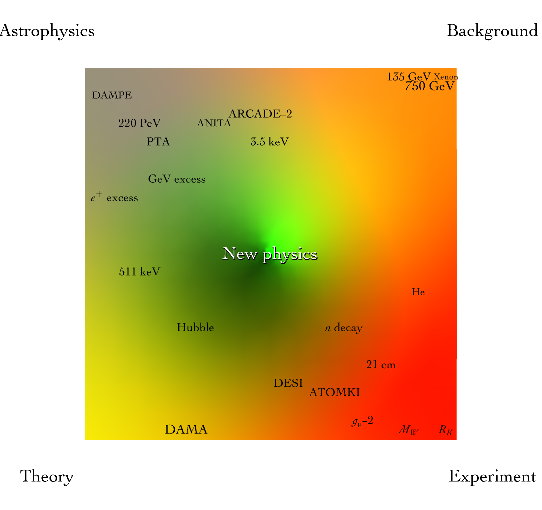
\includegraphics[width=\textwidth]{figs/AnomaliesSentiment}
\end{minipage}
\qquad
\begin{minipage}{0.30\textwidth}
\caption[Anomalies]{\label{fig:AnomaliesSentiment} 
\em Status map of recent {\bfseries anomalies} tentatively interpreted as Dark Matter or related to it. A confirmed discovery would appear in the central green region, while anomalies possibly affected by experimental (orange), backgrounds (yellow), astrophysical issues (black),
or by the lack of plausible theory (yellow) appear at the borders.}
\end{minipage}
\end{figure}


\begin{table}[p]
\hspace*{-1.5cm}
\small
\begin{tabular}{lllllcl}
\bf When & \multicolumn{2}{l}{\bf  Where} & \bf  Who & \bf What & \bf Stat   & \bf  Status\\ 
\rowcolor{yellow!20} 2025 & \ref{sec:220PeVanomaly}&\cite{220PeVanomaly} & {\sc Km3Net} & 
$E_\nu\sim 200\PeV$ & $2\sigma$ & astrophysics?\\
%
\rowcolor{green!5} 2024 & \ref{sec:DESIanomaly}&\cite{DESIanomaly} & {\sc Desi} & 
$w_{\rm DE}\neq -1 $ & $3\sigma$ & will be tested\\
%
\rowcolor{yellow!5} 2022 & \ref{sec:GRBanomaly}&\cite{GRBanomaly} & {\sc Lhaaso}/{\sc Carpet-2} & 
18 TeV/251 TeV $\gamma$ & ? & unclear\\
%
\rowcolor{red!50} 2022 &\ref{sec:CDFWmass} &\cite{WmassAnomaly} & {\sc CDF}& Too large $W$ mass & $7\sigma$ 
& disconfirmed\\
%
\rowcolor{yellow!20} 2022 & \ref{sec:COBCIB}&\cite{COBexcess} & {\sc Lorri} & 
Cosmic optic light excess & $4\sigma$ & disfavoured \\
%
\rowcolor{green!10} 2020 &\ref{sec:low:energy:DD:excess} &\cite{Low:energy:excesses} & {\sc Damic}& Low energy excess & $5.4\sigma$ 
& will be tested\\
%
\rowcolor{green!30}2020 & \ref{sec:NANOgrav}&\cite{PTA} & Pulsar Time Arrays 
& Stochastic gravity wave & $4\sigma$ 
& astrophysics?\\
%
\rowcolor{red!50}2020 & \ref{sec:XenonAnomaly}&\cite{XenonAnomaly} & {\sc Xenon1t} & $e^-$ excess recoils at 2.4 keV & $3-4\sigma$ 
& disconfirmed\\
%
\rowcolor{green!10} 2019 & \ref{sec:BHmassgap}&\cite{DMandBHmassgap} & {\sc Ligo}/{\sc Virgo} & BH in astro mass gap  & ? 
& will be tested\\
%
\rowcolor{green!10} 2018 & \ref{neutrontau}&\cite{NeutronBottleAnomaly} & Multiple experiments & $n$ decay to invisible  & $4\sigma$ 
& will be tested\\
%
\rowcolor{yellow!20} 2018 & \ref{sec:EDGESanomaly}&\cite{EDGES} & {\sc Edges} & 21 cm intensity & $3.8\sigma$ 
& will be tested\\
%
\rowcolor{green!10} 2018 & \ref{sec:ANITA}&\cite{ANITAanomaly} & {\sc Anita} & Upward CR around EeV & events 
& to be tested\\
%
\rowcolor{orange!20} 2017 & \ref{sec:DAMPE}&\cite{DAMPEexcess} & {\sc Dampe} & CR $e^\pm$ excess at 1.4 TeV & $2.6\sigma$ 
& fluctuation?\\
%
\rowcolor{green!10} 2017 & \ref{sec:dipoleanomaly}&\cite{dipoleanomaly} & Multiple surveys & CMB dipole vs distant matter & $\sim5\sigma$ 
& will be tested\\
%
\rowcolor{green!5} 2016 & \ref{sec:antiHeexcess}&\cite{Antihelium} & {\sc Ams} talks& CR $\overline{\rm He}$ & events 
& to be tested\\
%
\rowcolor{red!50} 2016 & \ref{sec:diphoton}&\cite{diphoton} & ATLAS and CMS & $\gamma\gamma$ peak at 750 GeV & $ 4\sigma$ & disappeared\\
%
\rowcolor{green!15} 2016 & \ref{sec:HubbleTension}&\cite{H0tension} & {\sc Planck} vs SN & Incompatible Hubble rate  & $3-6\sigma$ 
& to be tested\\
%
\rowcolor{red!50} 2016 & \ref{sec:S8}&\cite{S8anomaly} & $\Lambda$CDM fits vs local observations& $S_8$ matter inhomogeneity  & $3\sigma$ 
& disconfirmed\\
%
\rowcolor{red!30} 2015 & \ref{sec:Reticulumexcess}&\cite{Reticulumexcess} & {\sc Fermi} & $\gamma$-rays from the Ret II dwarf & $\sim3\sigma$ 
& not confirmed\\
%
\rowcolor{yellow!10} 2015 & \ref{sec:Atomki}&\cite{Atomki} & {\sc Atomki} & Boson at 17 MeV  & $7\sigma$  & not in MEG II\\
%
\rowcolor{orange!20} 2015 & \ref{sec:pbarexcess}&\cite{pbarexcess} & {\sc Pamela}, {\sc Ams} & CR $\bar p$ excess at 10-20 GeV & $\lesssim 2 \sigma$ 
& astro?\\
%
\rowcolor{red!50} 2014 & \ref{sec:RK}&\cite{RKanomaly} & LHCb & $R^{(*)}_K$ flavour ratios & $\lesssim 5\sigma$
& disconfirmed\\
%
\rowcolor{green!10} 2014 &\ref{sec:3.5keV}&\cite{3.5KeV} & $X$-ray telescopes & 3.5 keV $X$-rays & $4.4\sigma$ 
& will be tested\\
%
\rowcolor{red!50}2012 &\ref{sec:135GeVline}&\cite{135GeVline} & {\sc Fermi} & 135 GeV  $\gamma$-ray line & $3\sigma$ 
&disappeared\\
%
\rowcolor{red!20}2011 & \ref{sec:missingsatellite} &~\cite{toobigtofail} & Simulations vs Observations & Too big to fail & $?$ 
& astro?\\
%
\rowcolor{green!5} 2009 & \ref{sec:ARCADEexcess}&\cite{ARCADE2} & {\sc Arcade-2} & Excess isotropic radio emission & $>5\sigma$? 
& will be tested \\
%
\rowcolor{green!5} 2009 & \ref{sec:GCGeVexcess}&\cite{GeVGCexcess} & {\sc Fermi} & GeV $\gamma$-rays from the GC& $\infty$ 
& astro (sources)?\\
%
\rowcolor{yellow!20} 2008 & \ref{sec:positronexcess}&\cite{positronexcess} & {\sc Pamela}, {\sc Ams} & CR $e^+$ around 100 GeV & $\infty$ 
& astro (pulsar)?\\
%
\rowcolor{red!50} 2006 & \ref{sec:g-2}&\cite{muong-2measurements} & {\sc Bnl E821} & Muon magnetic moment & $5\sigma$ 
& lattice $\approx$ SM\\
%
\rowcolor{red!30}1999 & \ref{sec:DAMA}&\cite{DAMA} & {\sc Dama} & Seasonal variation & $13\sigma$ 
& not confirmed\\
%
\rowcolor{orange!20}199X & \ref{sec:cuspcore} & \cite{corecusp} & Simulations vs Observations & Cusp-core & $?$ 
& astro?\\
%
\rowcolor{orange!20}199X & \ref{sec:cuspcore} & \cite{diversity} & Simulations vs Observations & Diversity & $?$ 
& astro?\\
%
\rowcolor{red!30}199X & \ref{sec:missingsatellite} &~\cite{missingsatellite} & Simulations vs Observations & Missing satellites & $?$ 
& astro?\\
%
\rowcolor{yellow!20}1976 & \ref{sec:missingsatellite} &~\cite{satellite_plane} & Observations & Plane of satellites & $?$ 
& astro?\\
%
\rowcolor{orange!20}1970 & \ref{sec:511KeVline}&\cite{511KeVline} & Many & 511 keV $\gamma$-rays from the GC &$\infty$  
& astro?\\
\end{tabular}
\caption[Anomalies]{\em Recent {\bfseries anomalies} tentatively interpreted as Dark Matter or related to it.
\label{tab:anomalies}}
\end{table}










\section{Direct detection: current anomalies}

\subsection{The {\sc Dama/Libra} anomaly}
\label{DAMA}
\index{Anomaly!DAMA/Libra}
\label{sec:DAMA}
The amount of target material that can be used in a particular DM direct detection experiment 
is limited by the stringent requirements on background reduction. A larger target mass is useful only if a smaller relative background level can be achieved, so that one can still efficiently search for an excess of DM scattering events.
In late 1990s and early 2000s the {\sc Dama/Libra} experiment was able to use the world's largest detector mass by relaxing the background requirements and searching instead for an annual modulation in the DM direct detection signal in NaI crystals. At that time this also translated to world's leading sensitivity to spin-independent DM scattering, see fig.\fig{history:direct}.

As discussed in section~\ref{DMmodulation}, the rotation of the Earth around the Sun
causes a variation in the flux of DM particles hitting the Earth depending on the different periods of the year, 
such that the DM excess would peak around June 2.
The {\sc Dama} collaboration claimed the observation of an annual modulation with the expected phase.
The upgraded {\sc Dama/Libra} detector confirmed their earlier result 
improving the statistics and reaching a significance of roughly 13$\sigma$ for the cumulative exposure~\cite{DAMA,DAMA/LIBRA}, see fig.\fig{DAMAdata}.
A naive DM interpretation would need a spin-independent cross section of about $10^{-40}\cm^2$,
and a fit to the energy spectrum suggests a DM mass around $10\GeV$.



\smallskip

For a while both the {\sc CoGeNT} and {\sc Cresst} collaborations found anomalies possibly compatible with {\sc Dama}.
Subsequent experiments, however, ruled out this particular region of the parameter space.
Given the potential importance of the DAMA signal, a number of alternative models featuring additional DM properties that could enhance {\sc Dama}'s sensitivity relative to the other experiments, thus evading the bounds at the time, were explored: 
different couplings to $p$ and $n$, inelastic DM, multi-component  DM, DM scattering on electrons,  etc~\cite{DAMA_DMexplanations}.
However, as direct detection experiments advanced, they established orders of magnitude stricter bounds
(see fig.\fig{history:direct} and \fig{DDSIelec:bounds}),
rendering these proposed scenarios increasingly untenable.

\medskip

Although the {\sc Dama/Libra} anomaly seems no longer interpretable in terms of DM, the collaboration continues to support the claim of an anomaly. Various possible backgrounds and other (instrumental or environmental) effects that could account for the claim have been proposed~\cite{DAMAanomaly:alternatives}, and have been refuted by {\sc Dama}, see the {\sc Dama} papers~\cite{DAMA}.
The experiments {\sc Anais}~\cite{ANAIS} and {\sc Cosine}~\cite{COSINE}, which utilize NaI(Tl) crystals akin to {\sc Dama},  are investigating the same signal. 
First results by {\sc Anais} are consistent with no annual modulation in their counting rate, 
contradicting the {\sc Dama/Libra} claim at about $3\sigma$~\cite{ANAIS}.
Results from {\sc Cosine} also strongly constrain the {\sc Dama} claim, disagreeing with it at more than $3\sigma$~\cite{COSINE}.

\begin{figure}[t]
$$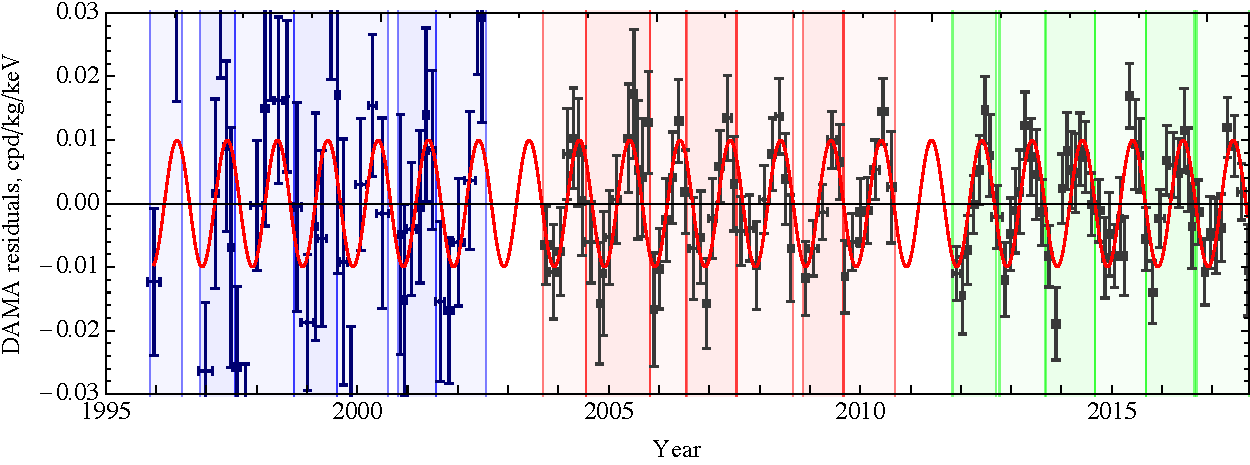
\includegraphics[width=\textwidth]{figs/DAMAmodulation}$$
\caption[DAMA data]{\label{fig:DAMAdata} 
\em The crosses represent {\bfseries DAMA data}: 
the residuals in the $2$-$6 \ {\rm keV}$ recoil energy window
computed by subtracting the average rates in the roughly annual
cycles chosen by DAMA  and plotted as  vertical bands.
The best fit to a Dark Matter signal (cosine annual modulation peaking at June 2) is denoted with a red curve.}
\end{figure}




\subsection{The {\sc Xenon1T} anomaly at 2.4 keV}
\label{sec:XenonAnomaly}
\index{Anomaly!2.4 keV}
In 2020 the {\sc Xenon1T} collaboration reported  an excess peaked at around 2.4~keV in the low-energy spectrum of electron recoil events~\cite{XenonAnomaly}. 
The local statistical significance was around  3-4$\sigma$, although already at that time it was suggested that part of this excess could be due to a small tritium background in the detector.
After implementing measures to mitigate tritium contamination, the successor {\sc Xenon}n{\sc T} experiment in 2022 did not observe the previously reported excess~\cite{XenonAnomaly}.

\medskip

During the interim, various dark matter-related explanations were proposed for the original observation~\cite{XenonAnomaly}:
\begin{itemize}
\item[$\circ$] The signal could have been due to new light particles 
created with keV energies in the Sun (the solar core has a temperature of a few keV) and then absorbed by electrons in the {\sc Xenon1T}  detector. 
However, this interpretation was disfavoured by the bounds on the cooling rates of hotter or denser stellar systems.

\item[$\circ$] DM as a scalar with a mass $M \approx 2.4\keV$ would produce a signal peaked at $M$, if absorbed by an electron in the detector.

\item[$\circ$] Particle DM elastically scattering on an electron would transfer enough recoil energy, if DM is fast, with $v_{\rm DM} \sim 0.1$
(or larger if $M < m_e$). 
DM faster than the galactic escape velocity
might be produced, e.g.,\ by DM semi-annihilations, or by DM scattering with the Sun.

\item[$\circ$] Inelastic scatterings of the usual slow (cold) DM on nuclei could produce a peak around 2.4~keV,
if the scattering is exothermic, i.e., into an appropriately lighter state.
\end{itemize}

\subsection{Low recoil energy excesses}\label{sec:low:energy:DD:excess}
The current direct detection experiments have reached sensitivities to sub-keV recoil energies.  At energies below 1 keV, some of these experiments are observing event rates that are well above the known backgrounds \cite{Low:energy:excesses}. The excesses were found in a number of experiments that use different target materials, types of sensors, surrounding holding structures, and are operating at different background levels. Some of these experiments are taking data on the surface, others in shallow underground facilities, and some in deep underground laboratories. It is highly unlikely that all the observed excesses are due to DM; 
however, some of them could be. That is, most of the observed excesses are most likely due to some not yet fully identified background source, with possible candidates as varied as: the cracking of the epoxy used to glue components of the detector, luminescence of the material in direct vicinity of the target material, transition radiation, excess neutron backgrounds, micro-fractures from the clamping of the detector, etc. 

\medskip 
Perhaps the most intriguing is the 5.4$\sigma$ excess of low-energy ionization events in the bulk of {\sc Damic}, {\sc Damic-M} and {\sc Sensei} skipper charge-coupled devices, housed in the {\sc Damic} cryostat at {\sc Snolab}, confirming the previous observation of the excess in the {\sc Damic} detector in 2020. At present there is no conventional instrumental explanation for the {\sc Damic} excess. Intriguingly, a DM particle with mass and
and cross section
\beq M\approx (2-4)\GeV,\qquad  \sigma_p\approx \text{few}~ 10^{-38}\,\text{cm}^2\eeq 
can explain the excess events. However, this DM explanation does require isospin-violating SI couplings, 
such that scattering on Ar largely or completely cancels
(the couplings to protons and neutrons need to have opposite signs). The explanation using isospin conserving SI couplings (the same couplings to protons and neutrons) is excluded by CDMSLite and by DarkSide-50. Similarly, DM spin-dependent  scattering is excluded by CDMSLite, LUX, and {\sc Picasso}~\cite{Low:energy:excesses}. 


\section{Indirect detection: current anomalies}\label{sec:IDanom}

\subsection{The {\sc Arcade-2} excess}\label{sec:ARCADEexcess}\index{Anomaly!{\sc Arcade}-2}
In 2009, the {\sc Arcade-2} collaboration measured the cosmic radio-wave emission over a wide range of frequencies. 
Above a few GHz the detected emission agrees  with the expected CMB signal. 
For frequencies between 22 MHz and a few GHz, however, the collaboration reported a significant excess \cite{ARCADE2}. 
Expressed in terms of the absolute temperature of the diffuse isotropic sky (see eq.~(\ref{eq:syncT})), the emission can be fit with $T(\nu) \simeq 1.2 \, {\rm K} \, (\nu/{\rm GHz})^{-2.60}$. 
The intensity of this excess emission is difficult to explain with known astrophysical mechanisms, such as the active galactic nuclei or star-forming galaxies, since it exceeds the flux predicted from astrophysical sources by a factor of approximately 5$-$6.
\medskip
 
Dark Matter has been proposed as a possible explanation \cite{ARCADE2}. 
DM annihilations in a large number of extragalactic halos may provide the additional source of $e^\pm$ 
that would emit synchrotron radiation (see section~\ref{sec:synchr}) and would power the emission detected by  {\sc Arcade-2}. 
The excess is found to be well fit by a rather conventional candidate: a DM particle with a mass $M \approx10 - 25\GeV$  
that annihilates into $\mu^+\mu^-$ (the measured hard synchrotron emission requires a hard $e^\pm$ spectrum, such as the one produced by a leptonic annihilation channel), with a thermal annihilation cross-section. 

A possible challenge to the DM interpretation, though, is the smoothness of the observed radio signal: the spatial fluctuations are very small, possibly inconsistent with DM annihilating in clustered structured at relatively low redshift, and annihilations at high redshift might be in conflict with the {\sc Edges} limits discussed in section \ref{sec:EDGESanomaly}. On the other hand, baryonic matter is also clustered and thus such a smoothness is also challenging for the proposed astrophysical explanations. 
 Alternative dark sector explanations have also been proposed, involving dark photons that oscillate into ordinary photons contributing to the radio background. Future radio-telescopes measurements, such as {\sc Ska}, will be needed to clarify the nature and the origin of the excess.


\subsection{The COB and CIB excesses}\label{sec:COBCIB}\index{Anomaly!{\sc Lorri}} \index{Anomaly!{\sc Ciber}}
The cosmic optical background (COB) consists of the total integrated light that has been emitted by all stars and galaxies over the history of the Universe, and that falls in the visible band. It can be estimated on the basis of galaxy counts, performed, e.g.,~with the Hubble Space Telescope ({\sc Hst}). 
Its detection, however, is challenging, because of the foreground provided by zodiacal light (sunlight scattered by local dust). 
The {\sc New Horizons} probe, a {\sc Nasa} mission dedicated to study the outer bodies of the solar system such as Neptune and Pluto, is in a good position to measure the COB, as zodiacal light is reduced at those locations.
The Long Range Reconnaissance Imager ({\sc Lorri}) instrument onboard {\sc New Horizons} has reported the COB's intensity to be $16.37 \pm 1.47$ nW m$^{-2}$ sr$^{-1}$ at the pivot wavelength of 0.608 $\mu$m~\cite{COBexcess}. 
This is a factor of 2 and about $4\sigma$ above the estimate from the {\sc Hst} galaxy counts. 

\medskip

\arxivref{2203.11236}{Bernal et al.~(2022)}~\cite{COBexcess} interpreted the excess 
in terms of axion-like DM particles with mass $M \simeq 5 - 25$ eV that decay into photon pairs. 
The required coupling is $g_{a\gamma\gamma} \sim \rm{few}/(10^{11}\GeV)$, 
which falls in the allowed window of the axion-like parameter space 
(axions are discussed in section~\ref{axion}:
see eq.\eq{gagammagamma} for the definition of $g_{a\gamma\gamma}$,
and fig.~\ref{fig:axion} for current bounds).
However, this interpretation is in strong tension with the measurements of the {\em anisotropy} of the COB. Since the DM distribution in the Universe is clumpy, the photon signal from decaying DM is expected to not be  isotropic. The predicted anisotropy is in contradiction with the upper bounds provided by the {\sc Hst}.

\medskip

Similarly, the Cosmic Infrared Background Experiment ({\sc Ciber}) reported an excess in the cosmic infrared background (CIB) radiation~\cite{CIBexcess}. This measurement is affected by larger uncertainties than the COB excess, mostly due to the relevance of the zodiacal light to the measurements of {\sc Ciber}, which is an Earth-based sounding rocket. 
The CIB excess has been interpreted in terms of $\sim2-3\eV$ axion-like DM particles decaying into photon pairs, with  coupling $g_{a\gamma\gamma} \sim 1.5 /(10^{10}\GeV)$. 
In this case the study of the anisotropy does not seem conclusive, 
but the larger coupling is in tension with stellar cooling bounds, see fig.~\ref{fig:axion}.



\subsection{The $X$-ray line at 3.5 keV}\label{sec:3.5keV}\index{Sterile neutrino}\index{Anomaly!3.5 keV}


\begin{figure}[t]
\begin{minipage}{0.36\linewidth}
\begin{center}
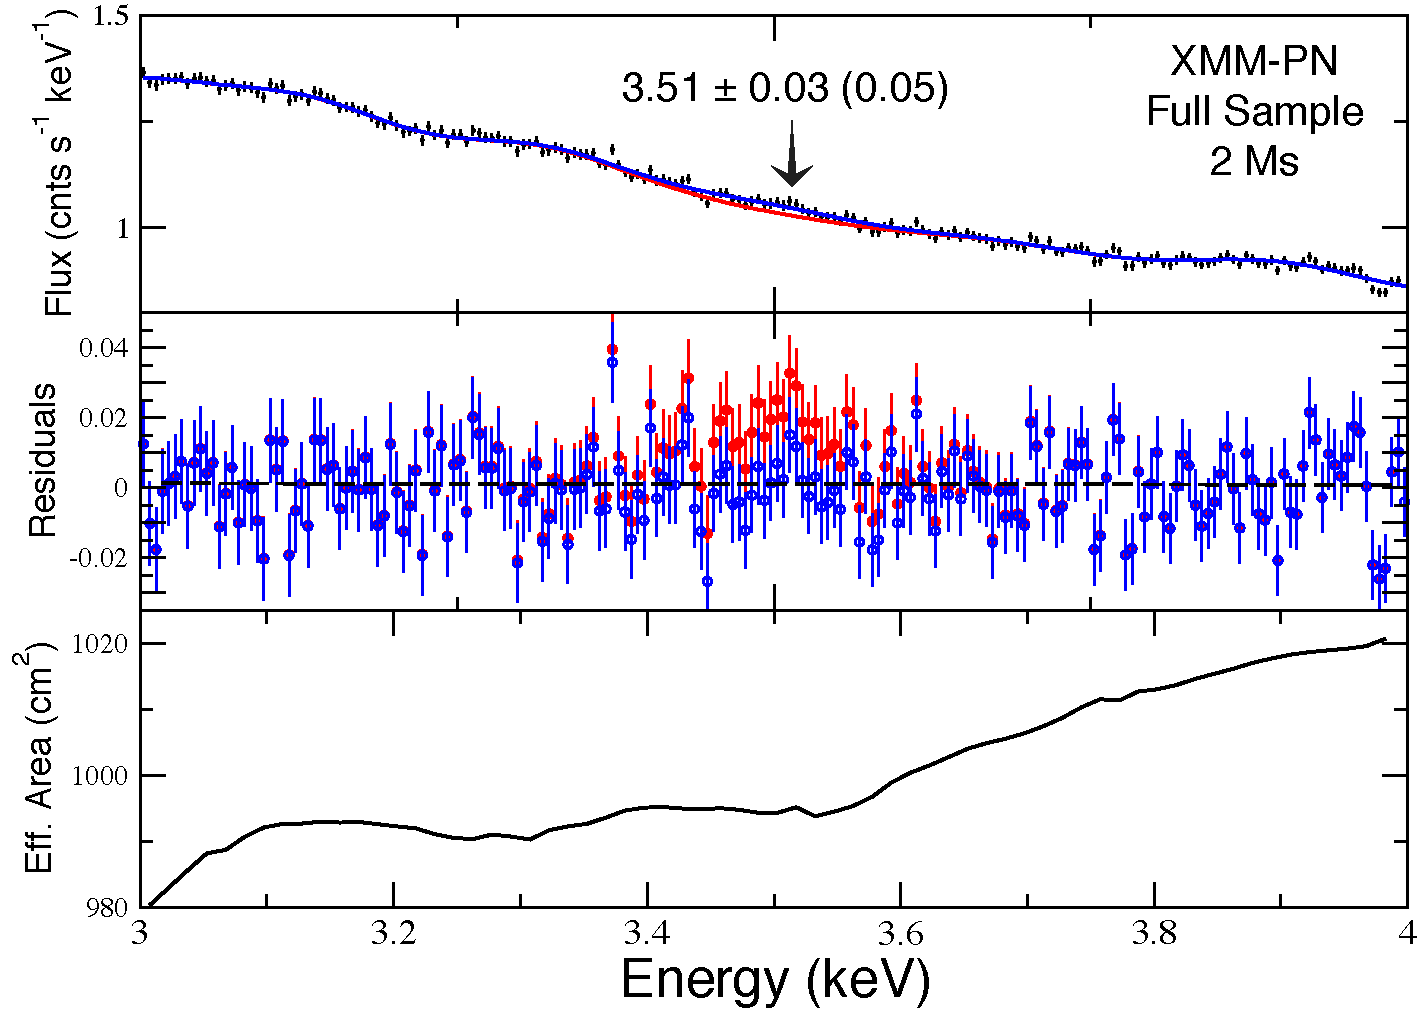
\includegraphics[width=\linewidth]{figs/3p5keV1.pdf}
\end{center}
\end{minipage}
\hfill
\begin{minipage}{0.36\linewidth}
\begin{center}
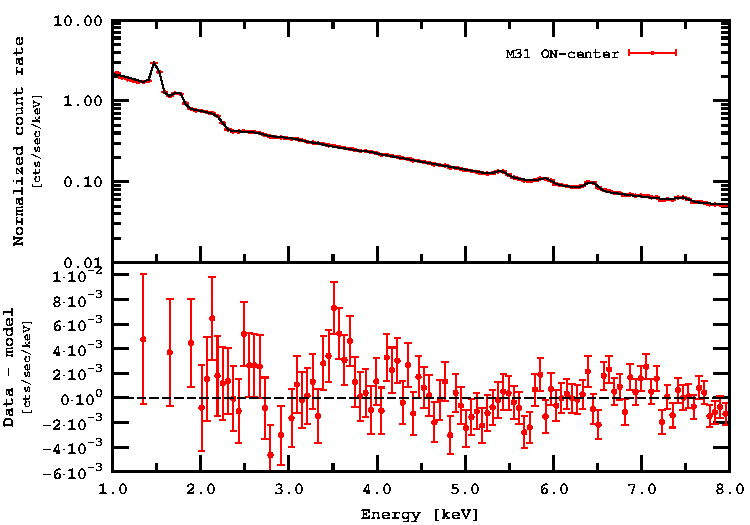
\includegraphics[width=\linewidth]{figs/3p5keV2.pdf}
\end{center}
\end{minipage}
\hfill
\begin{minipage}{0.26\linewidth}
\begin{center}
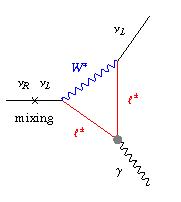
\includegraphics[width=\linewidth]{figs/NeutrinoSterileDecayFeynman}
\end{center}
\end{minipage}
\caption[The 3.5 keV line anomaly]{\em Left and Middle: {\sc Xmm-Newton} X-ray data from the Perseus cluster and the Andromeda galaxy 
on which the  {\bfseries claims of a 3.5 keV line} are mainly based (from Bulbul et al.~(2014), $\copyright$AAS, reproduced with permission, and Boyarsky et al.~(2014)~\cite{3.5KeV}, $\copyright$APS, reproduced with permission). 
 Right: Feynman diagram for the decay of a sterile neutrino, $\nu_R$, producing an X-ray $\gamma$ with energy equal to half of the $N_s$ mass.}
\label{fig:3.5keV}
\end{figure}


In 2014, \arxivref{1402.2301}{Bulbul et al.{}} and \arxivref{1402.4119}{Boyarsky et al.}~\cite{3.5KeV} both reported an independent detection of an $X$-ray line at $E_\gamma \simeq 3.55\keV$, cf. fig.~\ref{fig:3.5keV},
using observations from \textsc{Xmm-Newton} and \textsc{Chandra} of several galaxy clusters (notably, the flux from the Perseus cluster appeared to be anomalously high)
and of the Andromeda galaxy M31~\cite{3.5KeV}. 
Subsequent works claimed 
the same signal, albeit with varying degrees of significance, in various other targets: the Galactic Center, patches of the Milky Way halo, other --- but not all --- clusters, some `blank-sky' fields\ldots; and with other telescopes:   {\sc NuStar}, {\sc Suzaku}. 
At the same time, other studies claimed no detection, again in various regions: in the GC, patches of the MW halo, dwarf galaxies including Draco, stacked galaxies, individual clusters\ldots A reanalysis by \arxivref{2309.03254}{Dessert et al.~(2023)}~\cite{3.5KeV}, for instance, questioned even the very existence of the signal for the 3.5\,keV line in the data.
Given the complexity of the searches, the varied nature of the targets, and dependence on the modelling of the environments and the backgrounds, it is fair to say that while the detection and no-detection claims are in strong tension, they are not yet definitively contradictory.
The {\sc Hitomi} experiment~\cite{Hitomi}, which had the best energy resolution, did not observe the 3.5 keV line. Unfortunately, the gathered data was of very limited statistics since only slightly more than a month after launch in 2016 the satellite spun out of control and ultimately disintegrated.
Nevertheless, it did report a hint for a broadened excess at roughly the same energy.



\smallskip

Even if the 3.5\,keV line is truly present,
there is an ongoing debate whether it can simply be an unidentified atomic line emitted by excited interstellar and intergalactic gas. The intensely discussed possibilities are a potassium line and charge exchange reactions between sulfur and hydrogen. 


\smallskip


The 3.5\,keV line can be produced by $M\approx 7.1\keV$ DM particle decaying into $\gamma\gamma$ or $\gamma\nu$.  
A signal with approximately the correct strength, would, for instance, be obtained from $\gamma\nu$ decays of sterile neutrino DM, which was produced via non-resonant oscillations with mixing
angle
$\sin2\theta_{\rm mix}\approx 10^{-5}$ 
(section~\ref{FermionSinglet}). 
Such DM, however, would be too warm and thus not compatible with the Lyman-$\alpha$ bound in eq.\eq{WarmDMbounds}.
Different mechanisms that produce somewhat slower DM particles are phenomenologically more viable and would also help alleviate the anomalies in galactic sub-haloes and cores (section~\ref{sec:cuspcore}).

\smallskip

A feature that can discriminate between a DM and a non-DM origin of the signal is that in clusters of galaxies DM is predicted to have a significant velocity dispersion. DM decays would therefore produce a broader line than atomic emissions. This is quite intriguing in light of the {\sc Hitomi} hint mentioned above.\footnote{Since the DM speed is of the order of $10^{-3} c$, the broadening is expected to be of the order of $10^{-3} \, \, 3.55 \ {\rm keV} \simeq 3$ eV. This requires an exquisite energy resolution, which is, however, within the capabilities of {\sc Hitomi} and also of its successors.} 
Other DM-related explanations include the inelastic scattering of DM particles to an excited state that subsequently decays (`excited', `fluorescent' DM).

\medskip

Future X-ray surveys will be needed to shed light on the origin and precise features of the excess, 
e.g.,~the {\sc Athena} satellite~\cite{Athena}, {\sc Xrism} (the successor of {\sc Hitomi})~\cite{Xrism},
or the more futuristic {\sc Lem}~\cite{2211.09827}. 
A smoking gun of DM would be the detection of this excess in regions abundant in DM and scarce in gas, e.g., in
 dwarf galaxies. 
However, current searches in these regions have not yet yielded any positive results. 
Another unambiguous indicator would be to detect a Doppler shift of the line, with opposite signs in the east and west hemispheres of the Galaxy. Indeed, should the line originate from DM decays in the static DM halo, the motion of the solar system would cause an average blue shift in the signal coming from the hemisphere facing the direction of motion, and a red shift in the opposite direction.\footnote{Given the typical solar speed in the galactic frame, $v_\odot \approx 233$ km/s, such a shift in frequency is comparable to the broadening due to the DM peculiar velocity, and within the energy resolution of forthcoming instruments.}




\subsection{The $\gamma$-ray line at 511 keV}\label{sec:511KeVline}\index{Anomaly!511 keV}

\begin{figure}[t]
\begin{minipage}{0.32\linewidth}
\begin{center}
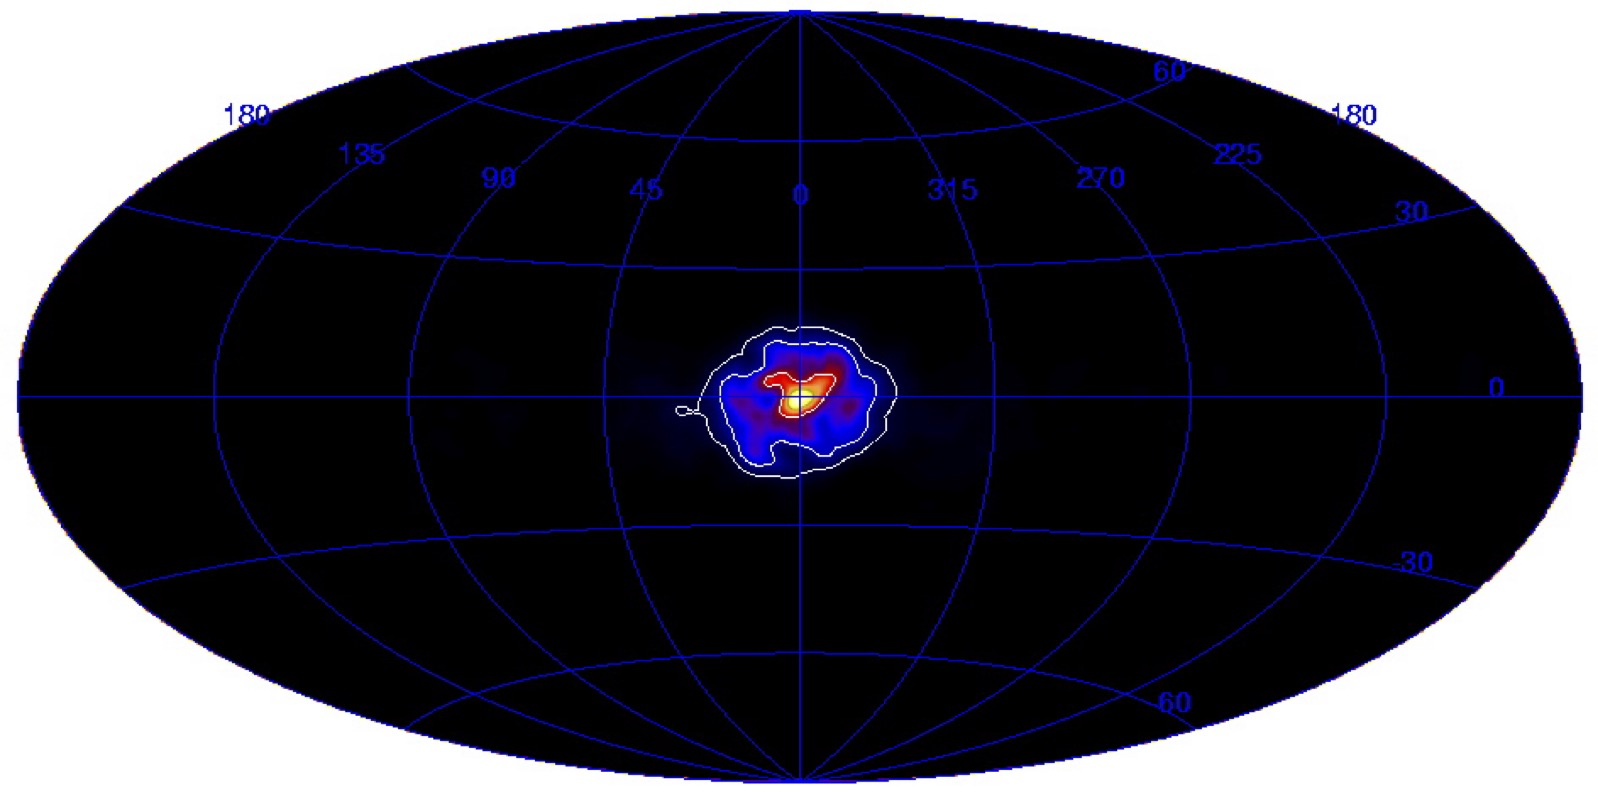
\includegraphics[width=\linewidth]{figs/511KeV1}
\end{center}
\end{minipage}
\hfill
\begin{minipage}{0.32\linewidth}
\begin{center}
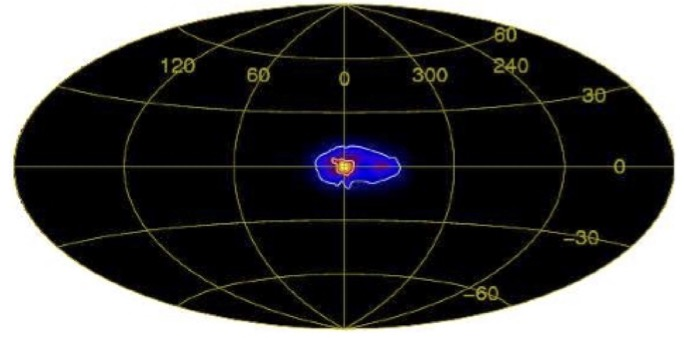
\includegraphics[width=\linewidth]{figs/511KeV2}
\end{center}
\end{minipage}
\hfill
\begin{minipage}{0.32\linewidth}
\begin{center}
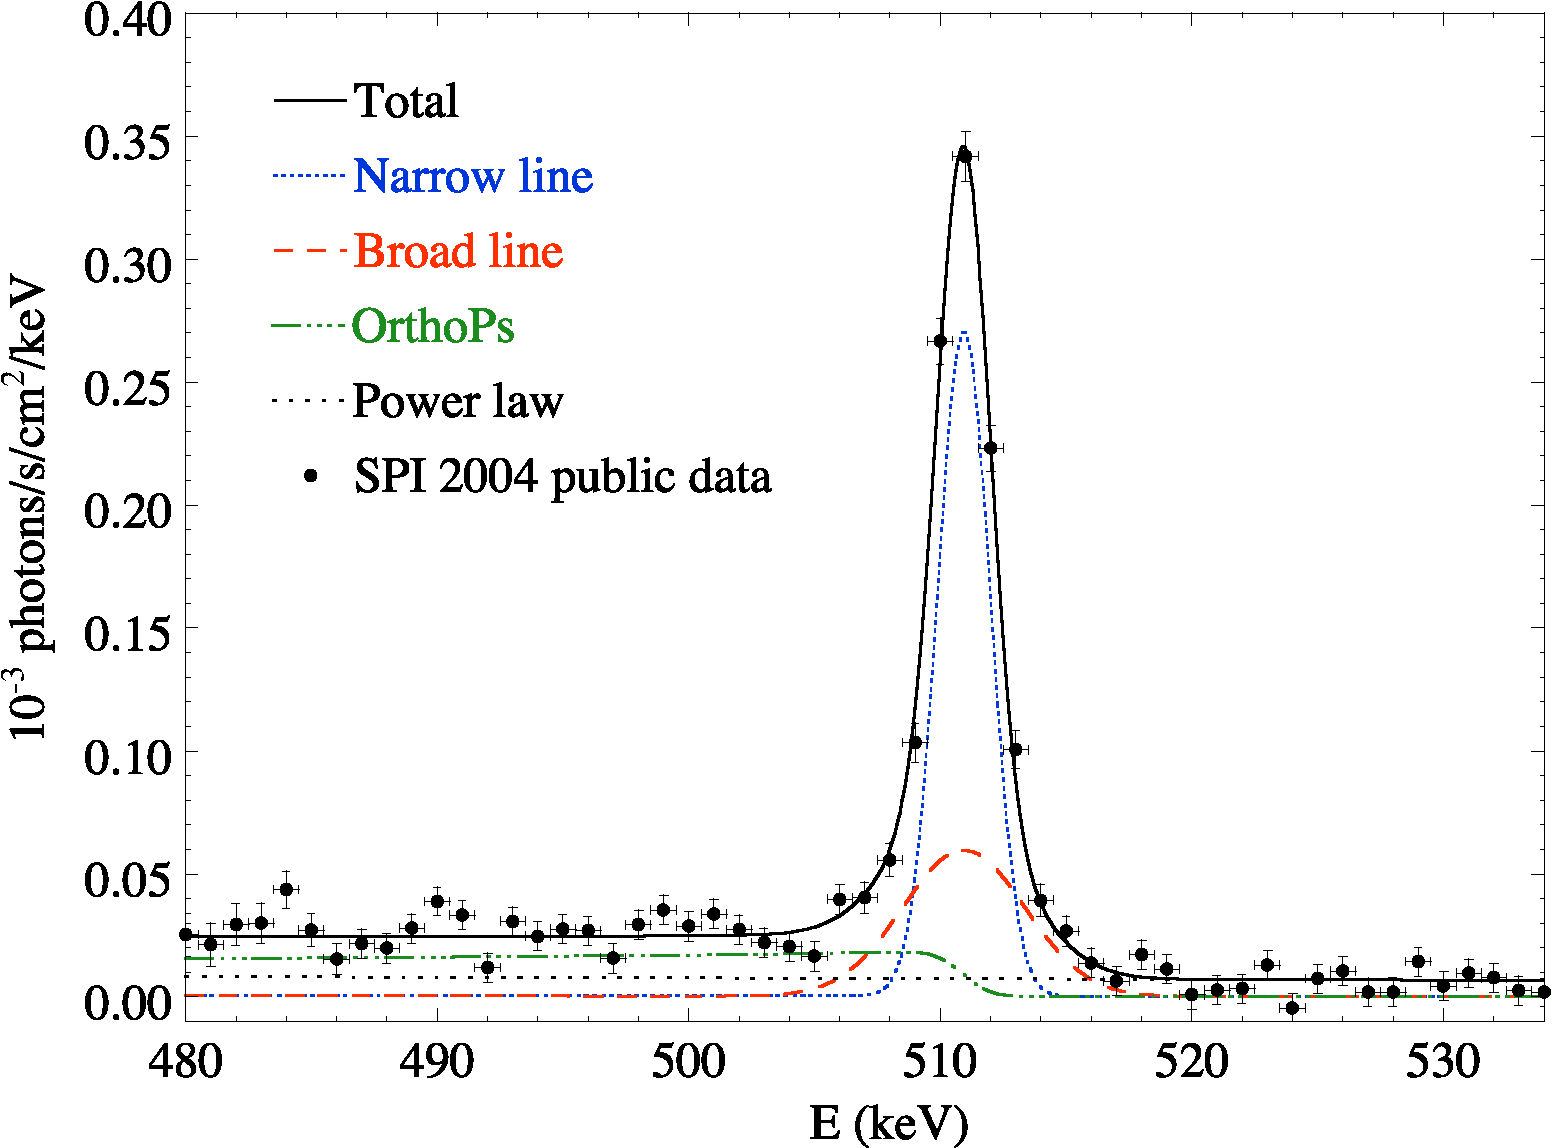
\includegraphics[width=\linewidth]{figs/511KeV3.pdf}
\end{center}
\end{minipage}
\caption[The $511\keV$ anomaly]{\em  Left: Initial {\bfseries 511 keV} map from {\sc Integral-Spi} data, showing the {\bfseries diffuse emission around the Galactic Center}. Middle: More detailed  $511\,{\rm keV}$, after 5 years of {\sc Integral-Spi} data, from which both a spherical bulge component and a  disk component can be extracted. Right: Spectral fit of the emission. The figures are, respectively, from Kn\"odlseder et al.~(2005), from the \href{https://sci.esa.int/web/integral/-/45328-integral-maps-the-galaxy-at-511-kev}{{\sc Integral} website} (see Weidenspointner et al.~(2008)) and from Jean et al.~(2006), in~\cite{511KeVline} ($\copyright$ESO, ESA/{\sc Integral}/MPE, reproduced with permission).}
\label{fig:511}
\end{figure}


A 511 keV emission coming from the region around the Galactic Center has been detected since the 1970's by a number of satellite and balloon missions~\cite{511KeVline}. The {\sc Integral/Spi} instrument has produced the most accurate measurements to date. Recently, the {\sc Cosi} balloon has also detected and started characterising this emission.

\medskip

The spectrum of the emission matches the expectations from $e^+e^-$ annihilations, as it peaks at $510.954 \pm 0.075$ keV,
which is precisely the electron mass. It is best described (see fig.~\ref{fig:511} right) as a superposition of two Gaussian components and a subdominant, lower-energy continuum. The first Gaussian is narrow (with width $\sim 1.3$ keV) and corresponds to direct $e^+e^-$ annihilation. The second Gaussian is broader (with width $\sim 5.4$ keV) and is expected when $e^+e^-$ annihilate after forming positronium in a gaseous environment. The continuum corresponds to the annihilation of ortho-positronium into 3$\gamma$. 


The measured flux implies the annihilation of $(2-5) \, 10^{43}\ e^+$ per second, corresponding to a remarkable instantaneous luminosity of about $\sim10^4$ times the luminosity of the Sun, or to the annihilation of $\sim 3 M_{\odot}$ over $10^{10}$ years, assuming a steady-state condition. 
The morphological analysis shows the superposition of two contributions: a somewhat spherical `bulge' and a fainter `disk' correlated with the galactic plane. The bulge extends to about 10$^\circ$ around the galactic center, while the disk has a vertical thickness of $4^\circ-7^\circ$ and a radial extent that does not go beyond  $|\ell| \approx 50^\circ$ longitude. The bulge/disk luminosity ratio is about 1.4.

\smallskip

The disk emission can be explained, at least in large part, by the $e^+$ injected by unstable nuclei produced in massive stars and supernovae, such as $^{26}$Al, $^{44}$Ti and $^{56}$Co. Alternative astrophysical explanations include fall-out from accretion onto the central black hole, X-ray binaries (the same ones possibly responsible for the GeV $\gamma$ excess from the GC, see section \ref{sec:GCGeVexcess}) and neutron star mergers. The bulge emission, however, can not be easily explained in terms of astrophysics, as it extends in latitude well beyond the region populated by stars. For this reason it has attracted a lot of attention, including explanations in terms of DM, which is naturally expected to be spherically distributed around the GC. An important constraint, both on DM models and on any other source of positrons, has been highlighted by \arxivref{astro-ph/0512411}{Beacom and Y\"uksel (2006)}~\cite{511KeVline}, who pointed out that the positrons must be injected with energies $\lesssim 3$ MeV otherwise they could annihilate `in flight' while still carrying  a lot of energy, producing an unobserved higher-energy gamma ray emission spectrum\footnote{Actually, \arxivref{2506.17427}{Kn\"odlseder et al.~(2025)} \cite{511KeVline} do claim the detection of such an in-flight annihilation signal in archival {\sc Comptel} data.  The $e^+e^-$ energy is reconstructed to be $\sim$ 2 MeV, in agreement with the Beacom and Y\"uksel constraint.}. 

\bigskip

The DM interpretations are mostly of two types:
light annihilating DM or de-exciting DM. A decaying DM explanation, on the other hand, seems to be disfavored as it gives too flat of a profile, with the predicted flux falling too slowly away from the GC. In the annihilation case, DM has to be lighter than about 3 MeV, given the Beacom and Y\"uksel constraint. Choosing for definiteness an NFW profile, the flux is fit with an annihilation cross section 
\beq \label{eq:sigmav511}
\langle \sigma v \rangle_{{\rm DM}\, {\rm DM} \to e^+e^-} \approx 5 ~ 10^{-31} \left(\frac{M}{3 \, {\rm MeV}} \right)^2 \, \frac{{\rm cm}^3}{{\rm s}}.\eeq
These values of mass and cross section are allowed by the CMB constraints (see section~\ref{sec:CMBconstraints}) 
but would, in minimal models, lead to a DM relic density that is too large (for thermal relic DM, the observed DM abundance requires an annihilation cross section in the early Universe which is 5 orders of magnitude larger that the one in eq.\eq{sigmav511}, see eq.\eq{sigmavcosmo}). 
Nevertheless, viable models can be constructed, e.g.~assuming that the cross section in eq.\eq{sigmav511} is $p$-wave suppressed, which implies then a less efficient suppression in the early Universe. 
The Beacom and Y\"uksel upper limit on the DM mass can also be slightly relaxed, e.g.~if the DM distribution at the GC features a pronounced density spike: this enhances annihilations, thereby requiring a cross section even smaller than eq.\eq{sigmav511} and thus suppressing the `in flight' contribution (\arxivref{2410.16379}{De la Torre Luque et al.~(2024)}~\cite{511KeVline}).

In the second category, heavier, WIMP-like DM particles are assumed to be collisionally excited to a state split by $\lesssim$ 3 MeV above the ground state. The subsequent de-excitation produces $e^+e^-$ pairs, of which the positrons subsequently annihilate with ambient electrons and produce the signal. TeV particles acquire a kinetic energy in the Galaxy of about 500 keV (given $v \sim 10^{-3} c$), which, if transferred to the excitation energy, is in the right ballpark to construct viable models.

\smallskip

The idea of checking the DM claim by searching for the same signal in dwarf satellite galaxies has so far given inconclusive results.



\subsection{The $\gamma$-ray GeV excess from the Galactic Center}\label{sec:GCGeVexcess}\index{Anomaly!GeV GC $\gamma$}
Since 2009, several authors have reported the detection of a gamma-ray excess from the inner few degrees around the GC, extending out to 10 or 20 degrees, at energies between 0.5 and 5 GeV~\cite{GeVGCexcess}. 
The spectrum and the nearly spherical morphology of the emission were found from the beginning to be compatible with the expectations from annihilating DM particles.
 One of the most detailed analyses is by 
 \arxivref{1402.6703}{Daylan et al.~(2014)}~\cite{GeVGCexcess}, which finds that 
  the excess has a high level of significance, and is 
best fit by a $\sim 45\GeV$ DM particle, distributed 
according to a contracted ($\gamma \simeq 1.26$) NFW profile, and annihilating into $b\bar{b}$ with 
a cross section $\langle \sigma v\rangle = (1.4 - 2) \times 10^{-26}$ cm$^3/{\rm s}$, 
which is compatible with the requirements for 
a thermal relic DM.\footnote{The astrophysical boost factor due to DM subhalos (see section \ref{sec:astroboost}) is typically not included in these analyses, hence the agreement between the two annihilation cross sections could be modified. However, in this case the boost factor is expected to be small, as discussed in section \ref{sec:astroboost}.
}
Fig.~\ref{fig:hooperon} shows both the earliest and one of the more recent fits to data. 
Thanks to the estimate of background modelling uncertainties quantified in \arxivref{1411.4647}{Calore et al.~(2014)}, it was soon realized that other good fits to the data are also possible, notably for DM annihilating into leptonic channels (pointing to lighter DM) and for gauge boson channels (pointing to heavier DM). 
The {\sc Fermi} collaboration  (\arxivref{1511.02938}{{\sc Fermi-LAT} coll.~(2016)}) essentially confirmed these findings, 
although doubts arose  given that similar excesses seem to appear elsewhere in the Galactic plane (\arxivref{1409.0042}{Calore et al.~(2015)}, \arxivref{1704.03910}{{\sc Fermi-LAT} (2017)}).

\medskip

It is important to bear in mind that  the identification of an `excess' 
 relies on the ability to carefully assess the background from  which the excess is hypothesized  to emerge. 
In the present case, the extraction of the residuals strongly relies on the modeling of the diffuse gamma-ray background (in particular the model made publicly available by the {\sc Fermi} collaboration)  as well as on additional modeling of astrophysical emissions. 
This includes emissions from {\sc Fermi} bubbles, isotropic component, unresolved point sources, molecular gas,... 
This `template fitting' strategy is subject to intrinsic uncertainties and prone to somewhat arbitrary modelization choices, hence it is often criticized.
Nonetheless, a consensus appears to exist that an excess relative to the expected templates is present.


\medskip

\begin{figure}
\begin{minipage}{0.48\linewidth}
\begin{center}
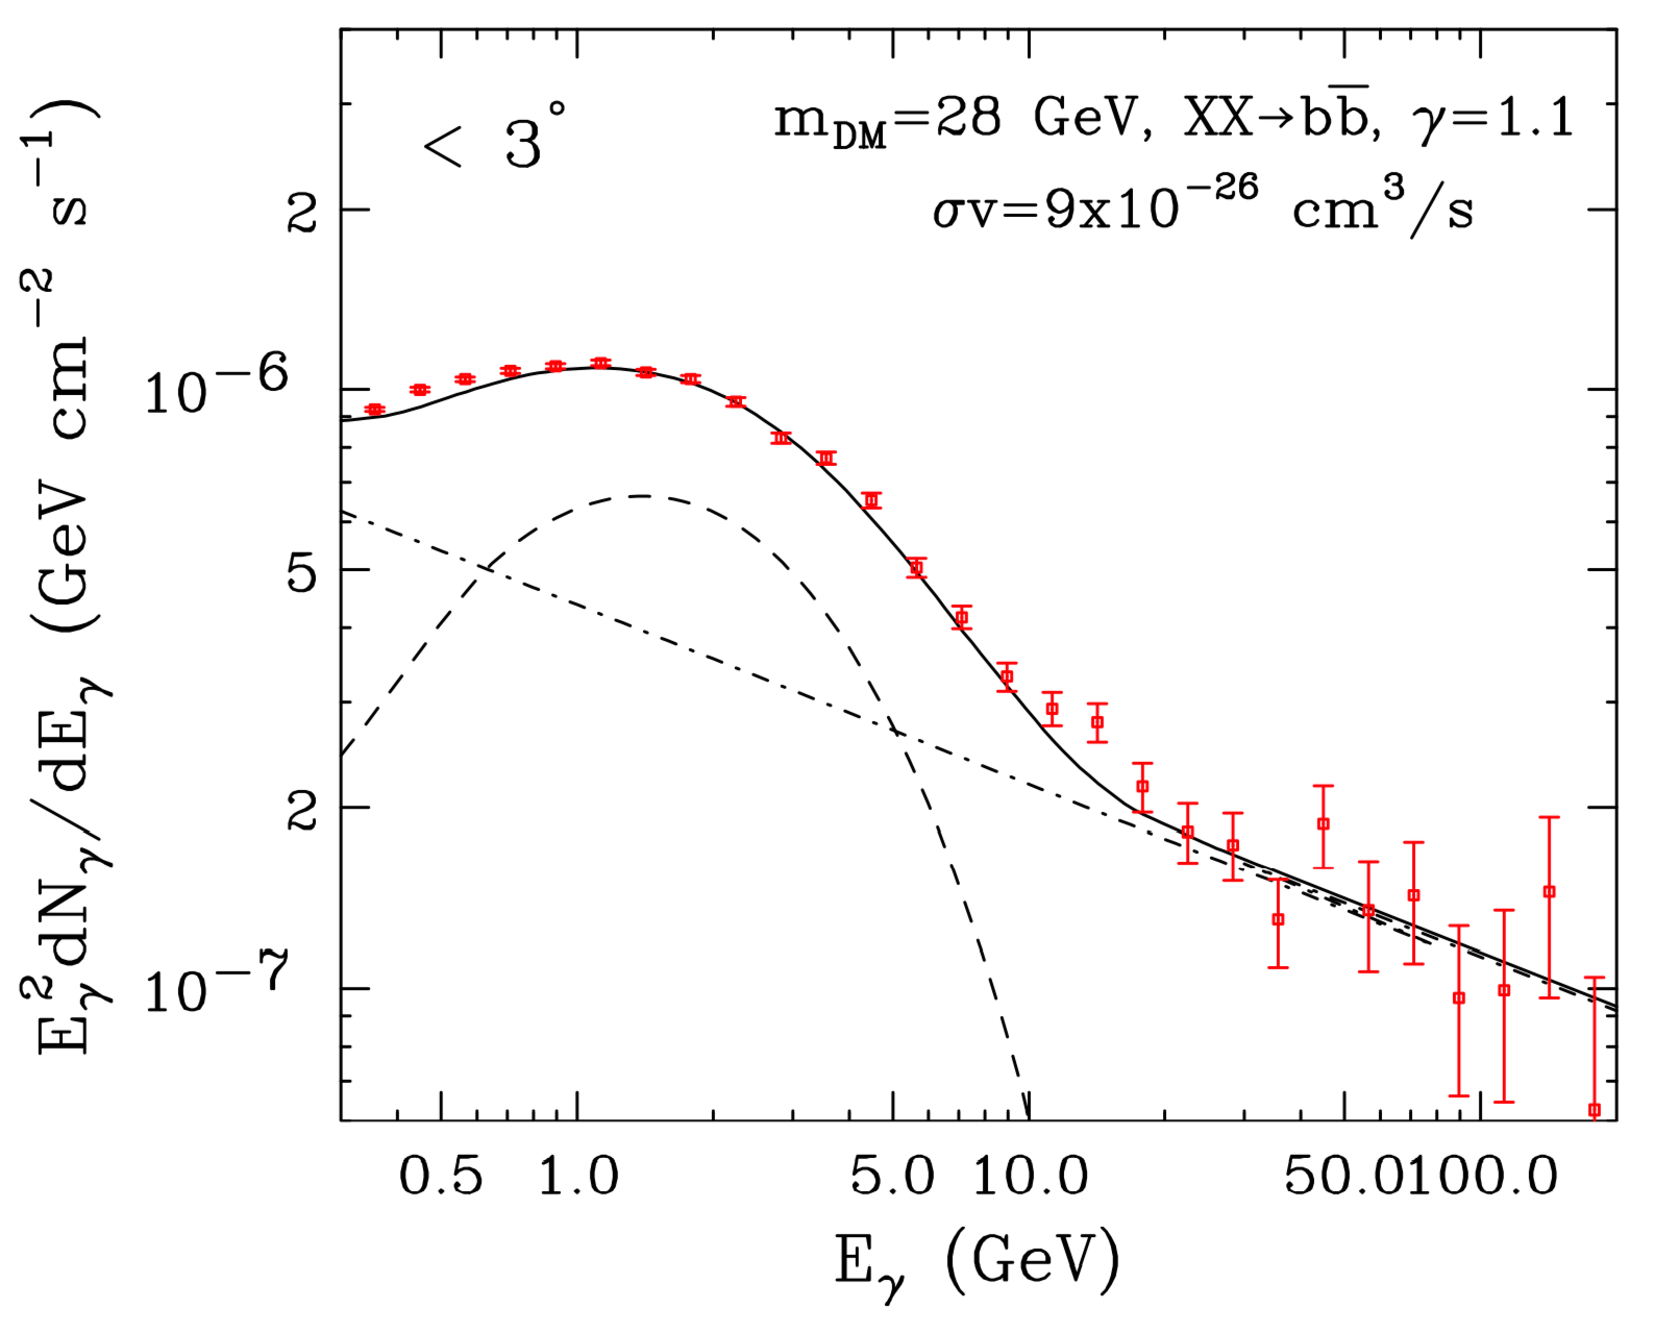
\includegraphics[width=\linewidth,height=7cm]{figs/hooperon1.pdf}
\end{center}
\end{minipage}
\qquad\hfill
\begin{minipage}{0.48\linewidth}
\begin{center}
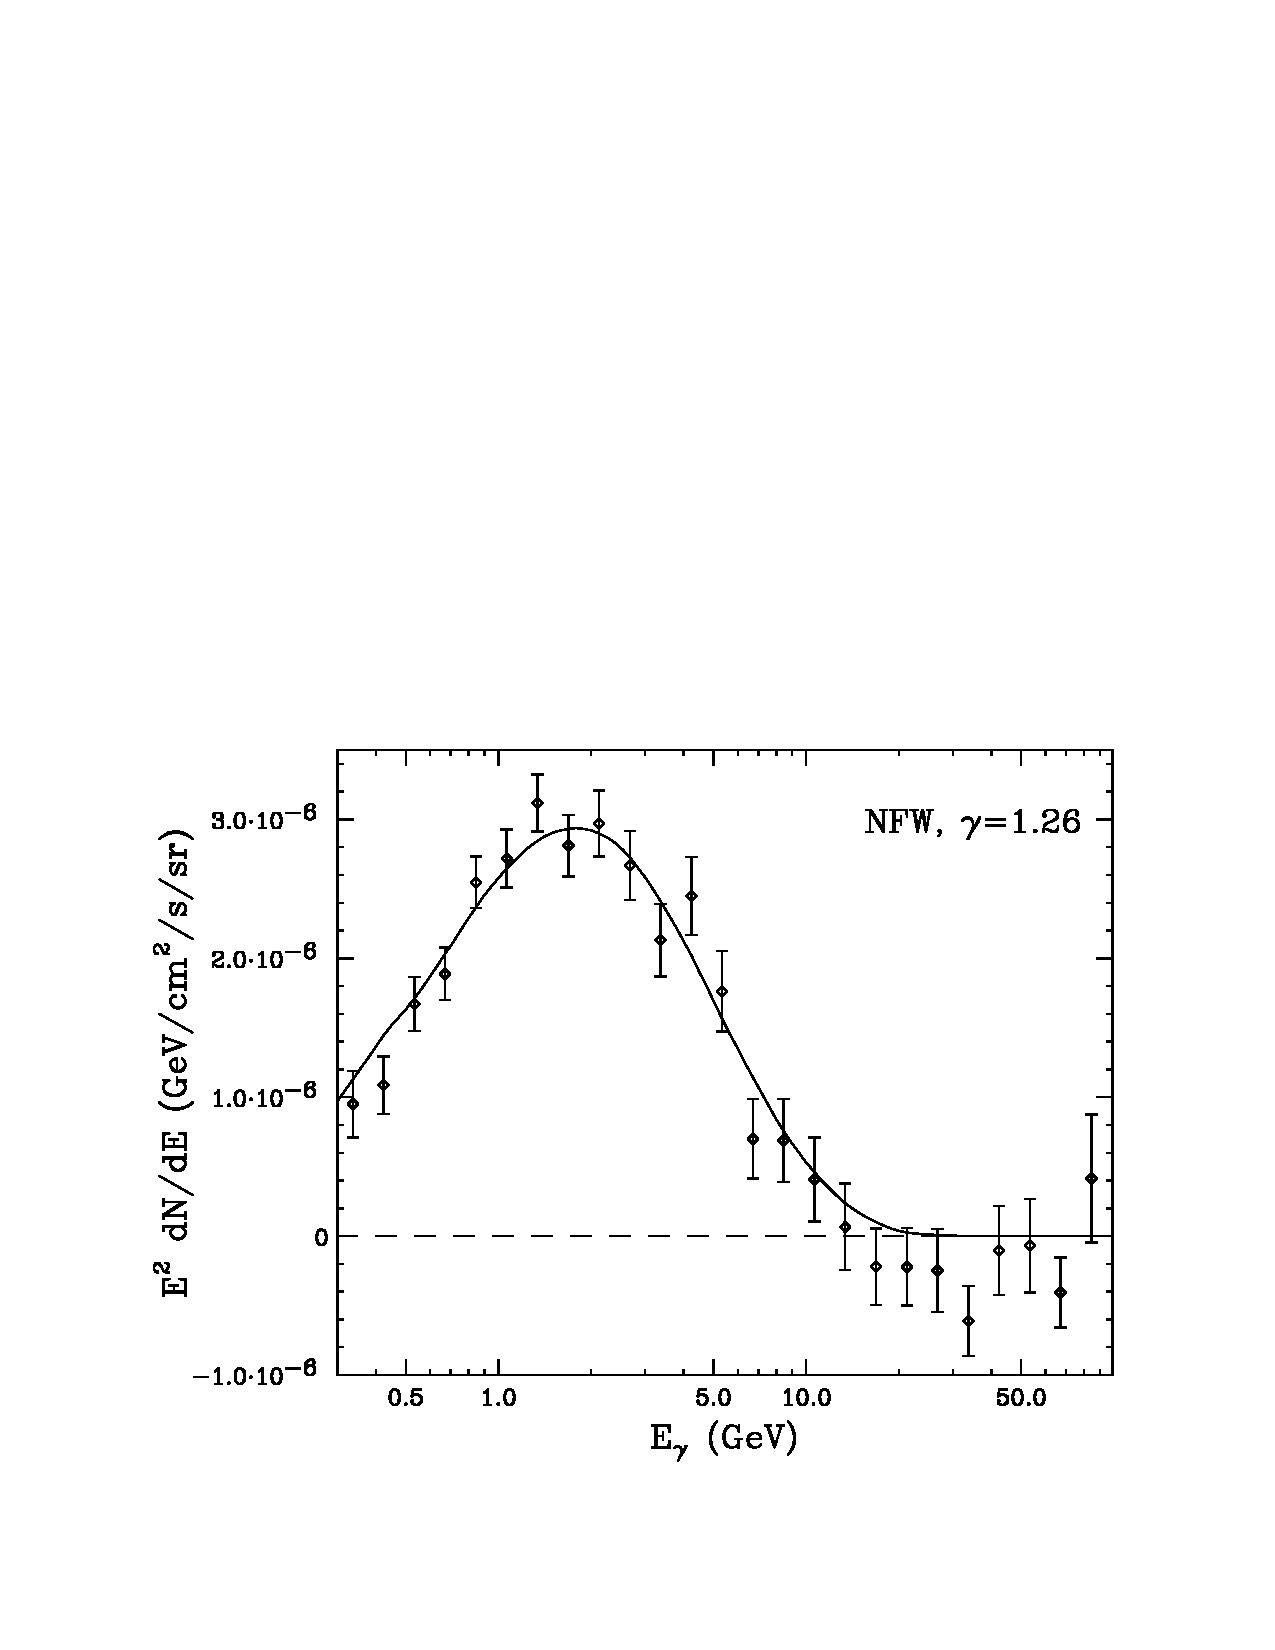
\includegraphics[width=\linewidth,height=7cm]{figs/hooperon2.pdf}
\end{center}
\end{minipage}
\caption[GeV excess from the GC]{\em \small The earliest (left) and the more recent (right) fits to the {\bfseries GeV $\gamma$ excess in the Galactic Center }for DM annihilation to $b\bar b$.  From \arxivref{0910.2998}{Goodenough \& Hooper (2009)} and \arxivref{1402.6703}{Daylan et al.~(2014)} in \cite{GeVGCexcess}.} 
\label{fig:hooperon}
\end{figure}

Before attributing the excess to DM one should consider possible alternative astrophysical explanations. 
A population of milli-second pulsars (MSP) has been a possibility from the very beginning. 
Initial detailed studies using wavelets analysis and photon-count statistics have shown that an interpretation in terms of a large number of unresolved point sources, such as MSPs, is statistically favored with respect to a diffuse emission (\arxivref{1506.05104}{Bartels et al.~(2015)} and \arxivref{1506.05124}{Lee at al.~(2015)}). 
This was later contested: \arxivref{1904.08430}{Leane and Slatyer (2019}, \arxivref{2002.12370}{2020)} questioned the robustness of the photon-count statistics method and revived the DM hypothesis (as did \arxivref{2006.12504}{List et al.~(2020)}),
while \arxivref{1908.10874}{Chang et al.~(2019)}, \arxivref{2002.12373}{Buschmann et al.~(2020)} and \arxivref{2102.12497}{Calore et al.~(2021)} maintain that MSPs are preferred. 
\arxivref{1611.06644}{Macias et al.~(2016}), \arxivref{1710.10266}{Bartels et al.~(2017)}, \arxivref{2402.05449}{Song et al.~(2024)} and others, on the other hand, argued in favor of a non-DM origin of the excess mostly on the basis of its morphology, which appears not to be completely spherical, and thus better correlates with the stellar population of the galactic bulge. 
\arxivref{2112.09706}{Cholis et al.~(2022)}, in contrast, argued against the MSP origin of the excess, since they observed a high-energy tail in the spectrum, which MSPs cannot produce.
\arxivref{2403.00978}{Holst and Hooper (2024)} also argued against the MSP option, claiming that {\sc Fermi} should have already seen dozens of MSPs, based on the luminosity function inferred from the observations (see also \arxivref{2507.17804}{List et al.~(2025)}). 
Indeed, directly detecting these putative MSPs remains a challenge, as their expected number is highly dependent on the assumed luminosity function, whose properties are mainly inferred from the detected MSPs within the Galactic disc (not the center).
Positive claims by the {\sc Fermi} Collaboration (\arxivref{1705.00009}{Ajello et al.~(2017)}) have later been corrected. 
Future telescopes, such as \textsc{Ska}, may offer more insight by detecting the associated radio emissions.
It might also be possible to detect them via their gravitational wave emissions: indeed, the high rotation velocities of pulsars make any irregularity in their shape a quadrupolar source of GWs (see \arxivref{1812.05094}{Calore, Regimbau and Serpico (2018)} and \arxivref{2507.05347}{Capdevilla (2025)}).


Other alternative interpretations include the possibility of a spectral break in the emission of the central Black Hole and the possibility that past isolated injections of charged particles (electrons or protons, in one or more bursts, possibly connected with the activity of the central Black Hole), can produce sufficient amounts of secondary radiation to account for the anomalous signal. 
While reproducing all the details of the observed excess might be not easy with these models, they represent additional plausible counterexamples to the DM interpretation.



\medskip

Testing the DM interpretation by searching for associated indirect detection signals is a challenging task. After various uncertainties are properly taken into account, neither the $\bar p$ constraints, the CMB observations, nor the $\gamma$-ray constraints from {\sc Fermi} observations of dwarf galaxies can conclusively confirm or refute the DM interpretation of the GC GeV excess. 
Similarly, testing the DM interpretation through direct detection or collider searches is not straightforward. This may seem surprising, given that the properties of the best fit candidate ($\sim 45\GeV$ DM coupling to quarks with weak-scale strength) na\"ively guarantee a signal at colliders and in nuclear recoil experiments. However, reality is more complicated,\footnote{See the discussion in section~\ref{sec:complementarities} for a more complete and general assessment.} and many `loopholes' are possible. For instance, indirect detection could proceed via a resonance in the $s$-channel, which would enhance the $\gamma$-ray signal but not the signals in direct detection and at the LHC. 
Indirect detection could also proceed via intermediate vector states, DM DM $\to VV \to b \bar b b \bar b$, 
where $V$ has a very small mixing with the SM photon. The $V$ decays into quarks, even if suppressed, will eventually occur on galactic scales and produce the $\gamma$-ray signal, while the direct detection scattering process, featuring the $V/\gamma$ mixing in the $t$-channel, would be extremely suppressed.
More systematically, several studies \cite{CoyDM}, working either in model-independent effective frameworks or in specific models,  have shown explicit examples in which Dark Matter can be `coy', meaning that it can have a single detectable signature (in this case the annihilation into $\gamma$-rays) while escaping all the other searches.


\medskip
\paragraph{Excesses from Andromeda?}
Given the interest garnered by the GC GeV excess, it is logical to speculate whether a similar signal might be detectable in our nearest galaxy M31 Andromeda~\cite{excessesM31}.
Intriguingly, the {\sc Fermi} satellite has detected gamma-ray emissions from Andromeda, where a `central, extended and symmetric' emission was found. However, its intensity is a factor of 5 higher than what would be expected for a signal consistent with the MW GC excess. Another study (\arxivref{1903.10533}{Karwin et al.~(2019,} \arxivref{2010.08563}{2020})) found evidence for an excess in the outer halo of Andromeda, roughly compatible in intensity and spectral shape with the MW GC signal. However, fitting it with DM requires a substructure boost factor of several orders of magnitude;  the same boost factor applied to the MW would predict overwhelmingly large emissions from the MW halo, in contradiction with observations.
 A few recent studies, on the other hand, find no Andromeda excess attributable to DM, and thereby only derive upper limits.



\subsection{A $\gamma$-ray excess from the Reticulum II dwarf galaxy?}\label{sec:Reticulumexcess}\index{Anomaly!Reticulum II}
In a period around 2015 it was claimed that several newly discovered dwarf galaxies (Reticulum II, and possibly Indus II, Tucana III and Tucana IV) could be showing a $\gamma$-ray excess around $2-10$ GeV, with up to $\approx3\sigma$ statistical significance~\cite{Reticulumexcess}. 
This was interpreted as annihilations of DM particles with estimates for DM mass ranging from a few GeV to a few hundred GeV, depending on the annihilation channel. The implied annihilation cross section was compatible with, or slightly higher than, the one required by DM as a thermal relic.
These characteristics also made the putative signal compatible with the $\gamma$-ray GeV GC excess, discussed in the previous section. 
The analysis by \arxivref{2212.06850}{Di Mauro et al.~(2022)} confirms the excess with similar significance, although other prior works had not~\cite{Reticulumexcess}.


\subsection{A $\gamma$-ray line at  135 GeV?}\label{sec:135GeVline}\index{Anomaly!135 GeV}

\begin{figure}[t]
\begin{minipage}{0.48\linewidth}
\begin{center}
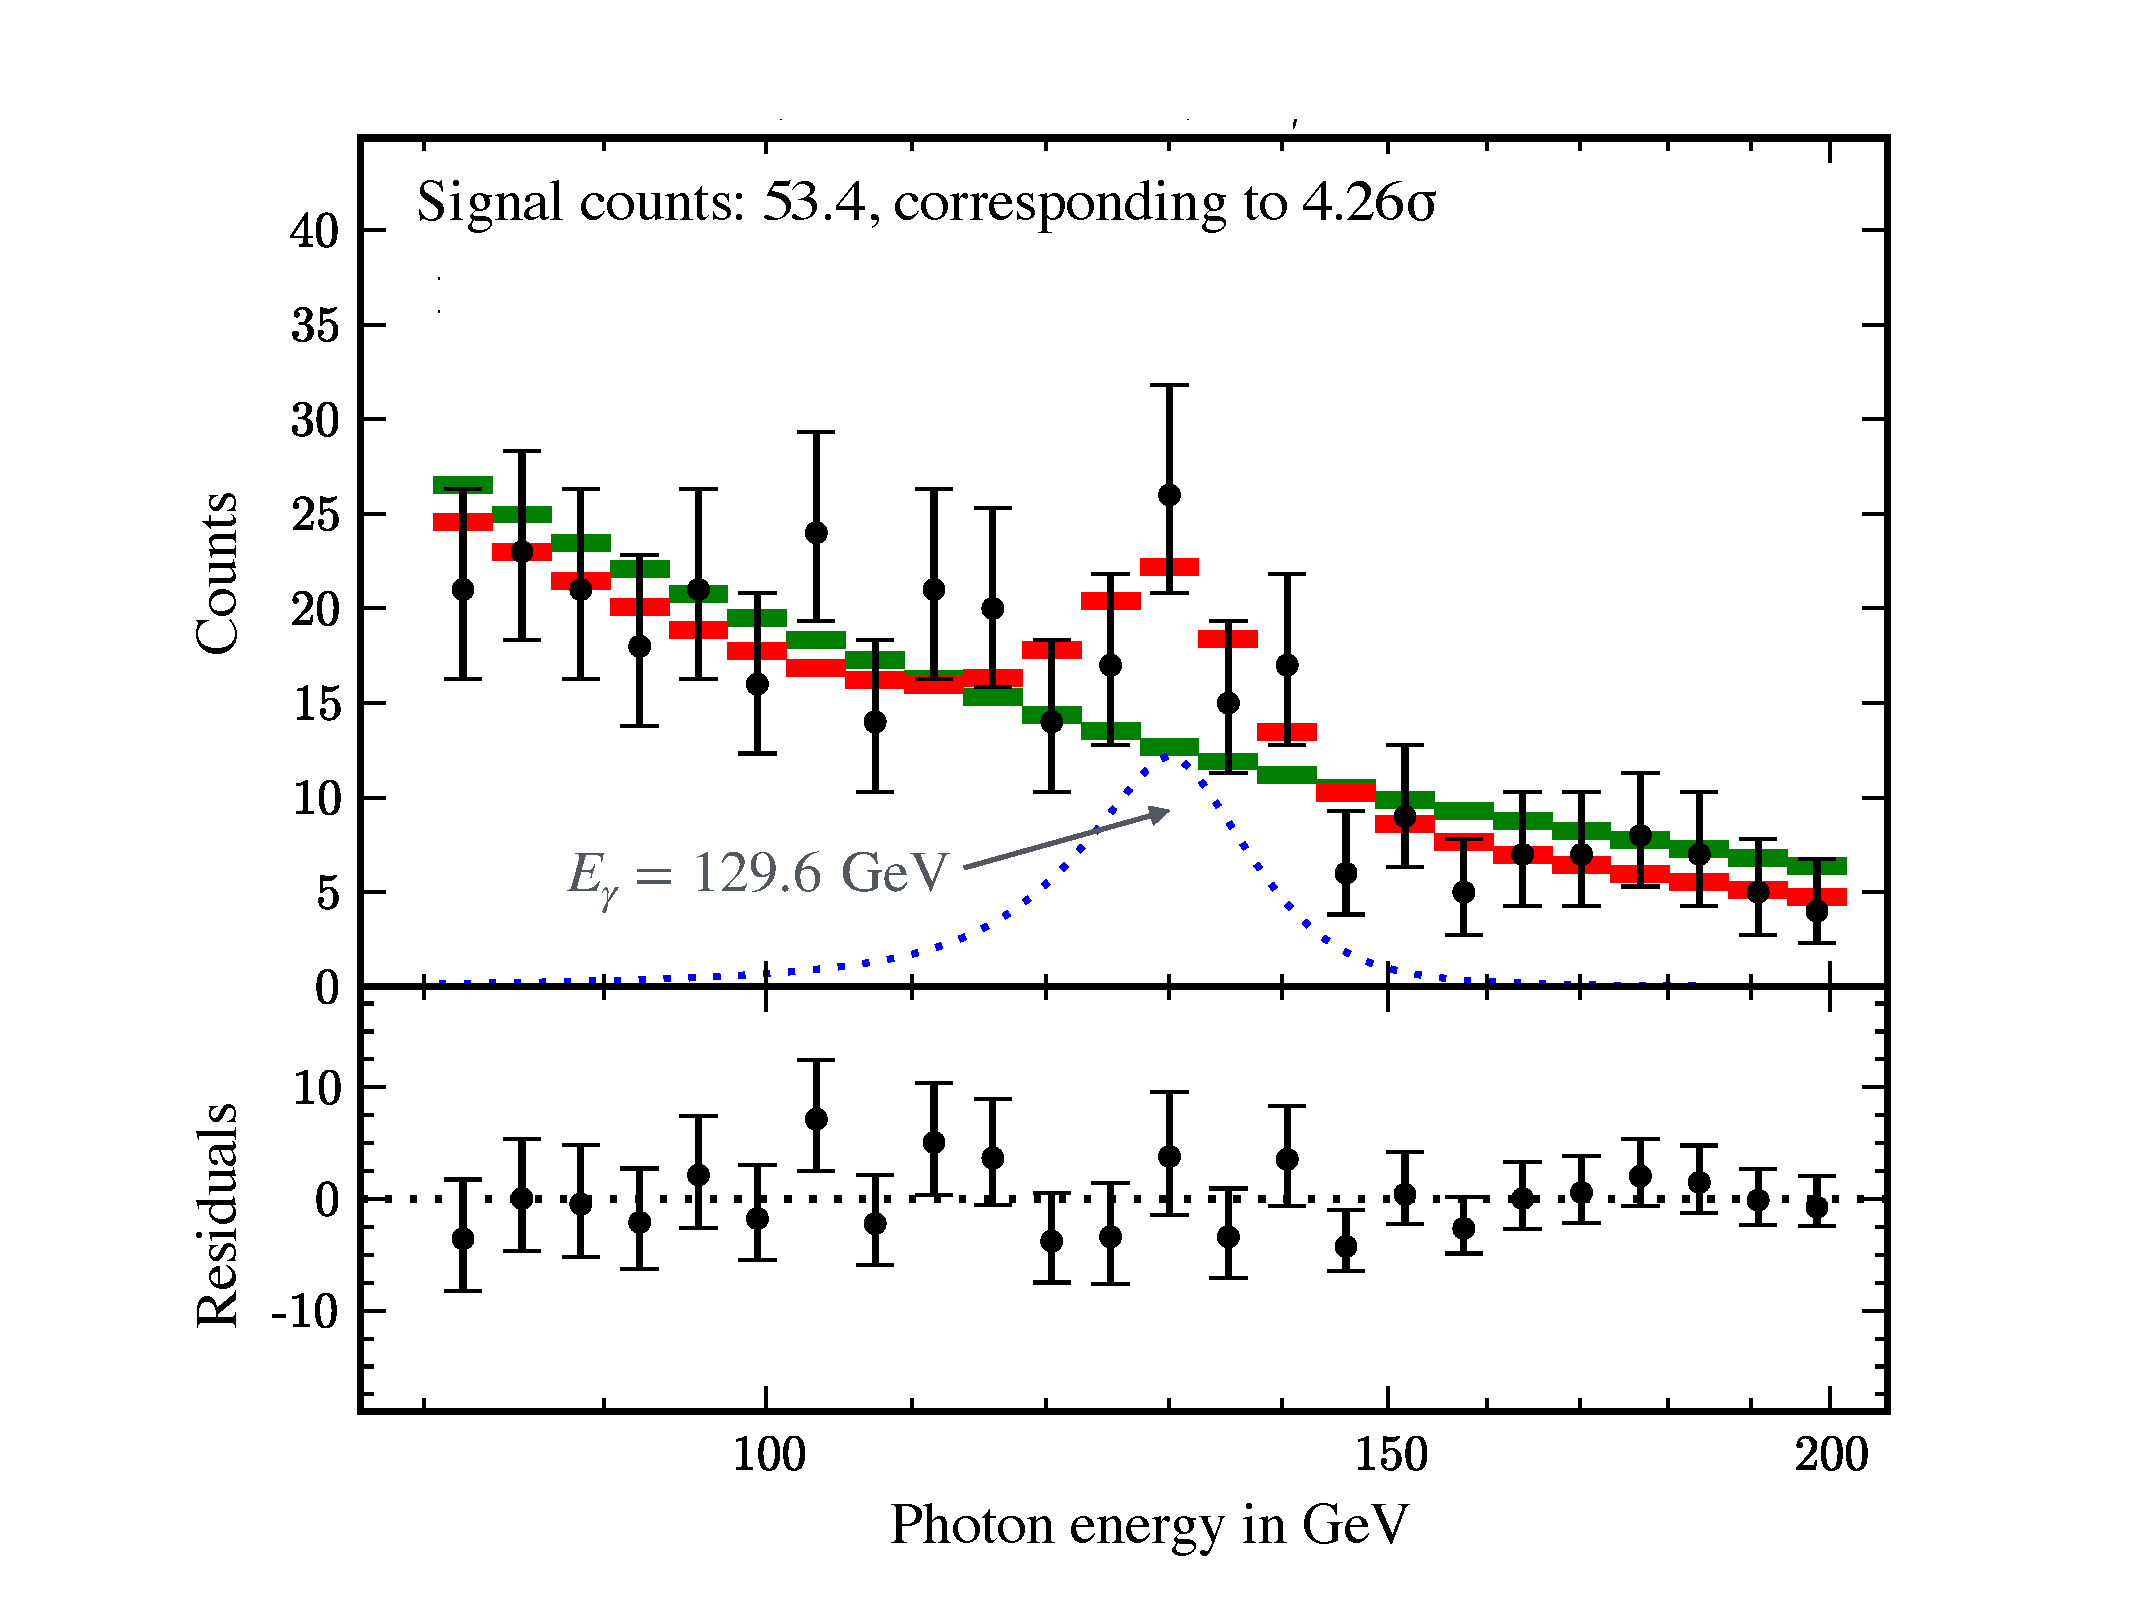
\includegraphics[width=\linewidth,height=7cm]{figs/fig_8point6_adapted_trimmed.pdf}
\end{center}
\end{minipage}
\hfill\qquad
\begin{minipage}{0.48\linewidth}
\begin{center}
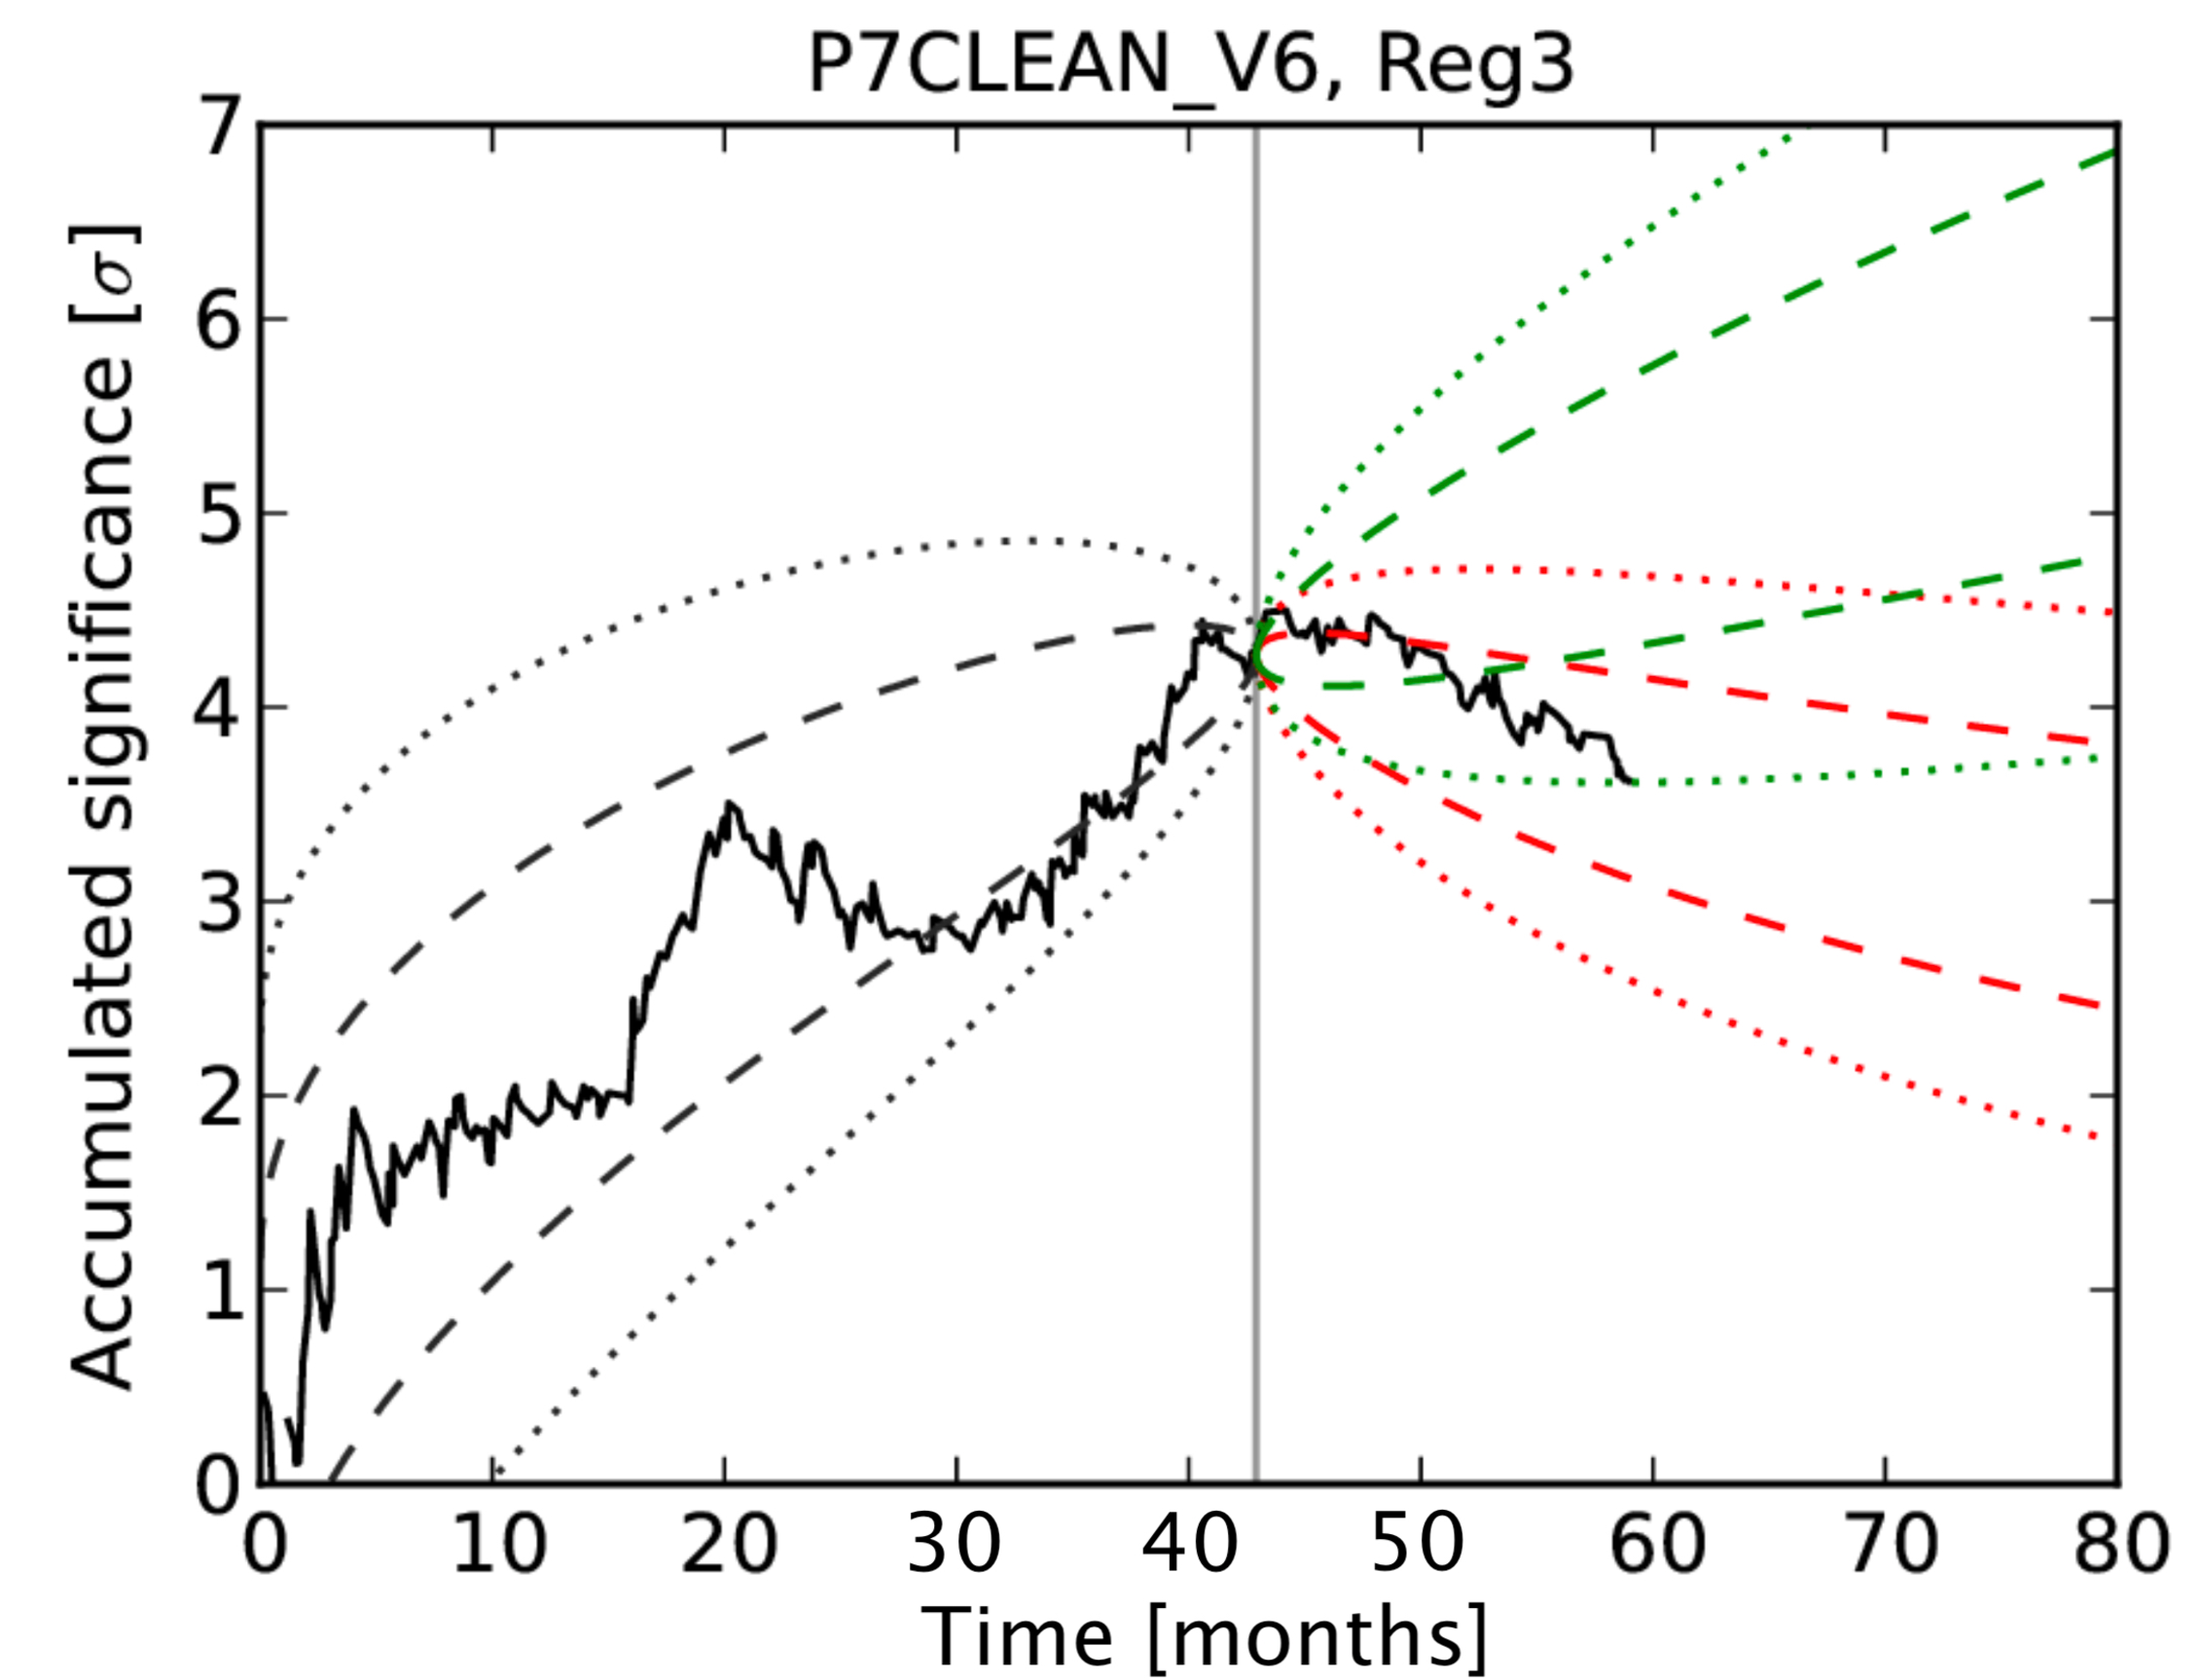
\includegraphics[width=\linewidth,height=6.5cm]{figs/wenigon2.pdf}
\end{center}
\end{minipage}
\caption[The 130 GeV anomaly]{\em Left: {\sc Fermi} $\gamma$-ray data and fits pointing to {\bfseries a line at about  130 GeV}. Right: behavior with time of the accumulated significance for this signal. 
The green lines correspond to the expected behavior of a real signal, with the dashed and dotted lines respectively associated with the 68\%CL and 95\%CL bands. The red lines trace the expected behavior of a statistical fluctuation. The black lines give extrapolations into the past for a constant source.
Left figure recreated from data in \arxivref{1204.2797}{Weniger (2012)}; right figure from Weniger (presentation at the {\sc Fermi} meeting, 2013)~\cite{135GeVline}.
}
\label{fig:wenigon}
\end{figure}


Around the years 2012-2013 a claim about a `135 GeV line' in the photon energy spectrum
gathered a lot of attention in the community~\cite{135GeVline}. 
It was originally identified by C.~Weniger and collaborators in the publicly available {\sc Fermi} data from an extended region that included the GC 
(the left panel in fig.~\ref{fig:wenigon} 
displays the most suggestive figure from the original analysis).
The claim was later supported by the results of other analyses,
with varying degrees of accuracy and claimed significance. The {\sc Fermi} collaboration (\arxivref{1305.5597}{Ackermann et al.~2013}), for instance, claimed a 3.3$\sigma$ (1.5$\sigma$)
local (global) statistical significance for the existence of the line.
Some studies observed the 135 GeV line in what could possibly be DM subhaloes of the MW and in galaxy clusters. 
Others found evidence of  two lines, at 111 GeV and 129 GeV. 
Still others challenged the analyses, proposing that the line(s) could have an unidentified instrumental, statistical or astrophysical origin. 



Tentative interpretations in terms of DM annihilation, and the associated DM model building, 
faced a 
significant challenge: if the line(s) were due to DM, it was plausible to expect an associated $\gamma$-ray continuum at lower energies, due to DM annihilations into other SM particles, as well as a signal in other CRs, such as anti-protons. 
The annihilation cross section into $\gamma\gamma$ required by the {\sc Fermi} data, $\sigma v\approx\mathcal{O}(10^{-27})\, {\rm cm}^3/{\rm s}$, 
would generically imply a large $\gamma$-ray continuum flux in conflict with existing bounds. 
This argument did not, however, exclude all possible DM models, as shown by explicit examples. 


\medskip

With more accumulated data  the signal significance diminished (see the right panel in fig.~\ref{fig:wenigon}), thereby indicating 
that this was probably not an actual signal. An understanding gradually developed that the line had been a combination of an instrumental effect and a statistical fluctuation. The \arxivref{1506.00013}{2015 {\sc Fermi}} analysis of an increased and improved dataset~\cite{Ackermann:2015lka} put the claim to its final rest as the local significance dropped to $0.7 \sigma$. Additionally, the \arxivref{1609.08091}{2016 {\sc Hess}} search~\cite{1609.08091} also independently excluded it (albeit barely).




\begin{figure}[t]
\begin{center}
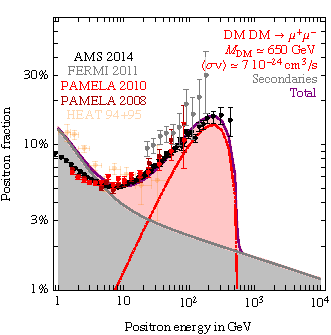
\includegraphics[width=0.31 \textwidth]{figs/CRdata_positron_excess} \quad
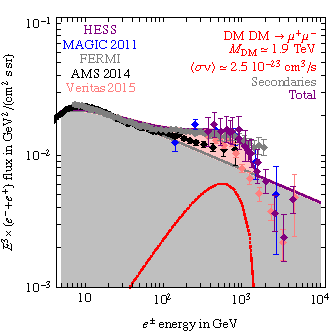
\includegraphics[width=0.31 \textwidth]{figs/CRdata_lepton_excess} \quad
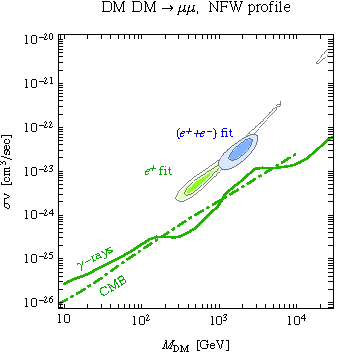
\includegraphics[width=0.31 \textwidth]{figs/positronexcess_fit.pdf} 
\end{center}
\caption[The {\sc Pamela}/{\sc Ams} positron excess and its (annihilating) DM interpretation.]{\em \label{fig:positronexcess} The {\bfseries  {\sc Pamela}/{\sc Ams} positron excess} and its DM interpretation, circa 2015. Left: The annihilating DM fit of the rising positron fraction, featuring a leptophilic DM with a mass slightly below 1 TeV and a very large annihilation cross section.  Center: The DM fit of the $e^++e^-$ flux, featuring a slightly heavier DM and an even larger annihilation cross section. Right: The regions in the DM parameter space preferred by the fit to only the positron fraction (green), and a fit to the $(e^++e^-)$ flux (blue), with contours denoting the $3\sigma$ and 5$\sigma$ regions. The constraints from $\gamma$-rays (solid line) and the CMB (dot dashed) are those discussed in section~\ref{sec:IDconstraints}.}
\end{figure}



\subsection{The {\sc Pamela}/{\sc Ams} positron excess}\label{sec:positronexcess}\index{Anomaly!{\sc Pamela}/AMS}
In 2008, data from the {\sc Pamela} satellite~\cite{Adriani:2008zr,Adriani:2010ib}  revealed a
steepening of the energy spectrum of the cosmic ray positron fraction, $e^+/(e^+ +e^-)$, above 10 GeV and up to 100 GeV 
(below $\sim10$ GeV the situation is more involved, since  the Sun distorts and modulates the inter-stellar spectrum, see page  \pageref{solar_modulation}). 
This behaviour had  previously been hinted at by the {\sc Heat} balloon experiment \cite{Barwick:1997ig} and 
later confirmed by the {\sc Fermi} satellite \cite{FermiLAT:2011ab} and the {\sc Ams} detector \cite{AMSpositrons2013,AMSpositrons2014}. 
{\sc Ams} in particular extended the data to several hundreds GeV,\footnote{Published data on the positron fraction go up to 500 GeV, while for the $e^+$ flux they reach 1 TeV.} identifying a possible flattening above 300 GeV.
The data, shown in fig.\fig{positronexcess} (left), has the typical shape one would expect from DM, see the discussion in section~\ref{chapter:indirect}, in particular
fig.\fig{DMIDcartoon}.





\smallskip

Given that the positron fraction in CR data grows with energy to almost $20\%$, interesting information may be provided
also by the experiments that cannot discriminate $e^+$ from $e^-$, but are able to measure
the  energy spectrum of the electron--positron sum, $(e^++e^-)$, to higher energies. For this, 
several experiments performed around the same time showed hints of an anomalous `bump' at a few TeV, 
possibly due to the same physics that generated the $e^+/(e^+ +e^-)$ excess, see  fig.\fig{positronexcess} (center).
Both the {\sc Fermi} satellite~\cite{FERMIleptons} and {\sc Ams}~\cite{Aguilar:2014fea} obtained a fairly featureless spectrum up to 1 TeV.\footnote{After initial mild disagreement in the spectral indexes ({\sc Ams} being steeper), the {\sc Fermi} collaboration released new Pass 8 data in 2017~\cite{Abdollahi:2017nat}, which brought its data points closer to those of {\sc Ams}.} 
Above 1 TeV, data from the ground based Imaging \v Cerenkov telescopes {\sc Hess}~\cite{HESSleptons}, {\sc Magic}~\cite{BorlaTridon:2011dk} and {\sc Veritas}~\cite{Staszak:2015kza} indicated a potential cutoff or a steepening of the spectrum at energies of a few TeV. Subsequently, the {\sc Calet} and {\sc Dampe} collaborations also presented data: {\sc Calet} in agreement with {\sc AMS}, while {\sc Dampe} obtained a higher flux and steeper spectrum, see section~\ref{sec:DAMPE} for further discussion. 


In contrast to these intriguing excesses in the leptonic sector, data from {\sc Pamela} \cite{PAMELApbar} (and, much later, {\sc Ams} \cite{Aguilar:2016kjl}) exhibited no anomalies at comparable energies in antiprotons. A compilation  of the relevant data is shown in fig.~\ref{fig:CRdata}. 




\medskip

The $e^+$ and $(e^++e^-)$ results deviate rather spectacularly from the power-law behavior expected from the cosmic ray propagation models.  Importantly, they imply the existence of a source of {\em `primary'} $e^+$ (and $e^-$) beyond the already expected astrophysical sources.\footnote{Simple kinematic arguments predict that the spectrum of any {\em secondary} positrons should decrease  much more steeply than observed, see \arxivref{1108.4827}{Serpico (2012)} \cite{positronexcessastro}. In this context, {\em primary} refers to the charged CRs produced directly by some (astrophysical or exotic) source while {\em secondary} refers to the CRs generated as byproducts of primaries colliding with the gas particles of the interstellar medium.} 


\subsubsection*{DM interpretations}
Quite naturally, DM annihilations (or decays) were immediately proposed as such a source~\cite{positronexcess}. 
It was quickly realized that in order for DM to fit the data, the DM particle had to: 
\begin{itemize}
\item[$\triangleright$] Have a mass in the TeV to multi-TeV range, to reproduce the feature in the $(e^++e^-)$ spectrum.
\item[$\triangleright$] Have an annihilation cross section of the order of $\sigma v\approx10^{-23}\, {\rm cm}^3/{\rm s}$ or larger, in order to produce large enough $e^\pm$ flux to fit the positron rise and the $(e^++e^-)$ bump.
This cross section is significantly higher than the annihilation cross section required for a thermal relic, $\sigma v \approx 2 \, 10^{-26}\, {\rm cm}^3/{\rm sec}$, see eq.~(\ref{eq:sigmavcosmo}). 
\item[$\triangleright$] Be leptophilic, i.e.,
predominantly annihilate (or decay) into leptons to avoid contradicting the absence of an anomaly in antiprotons.
\end{itemize} 
Fig.~\ref{fig:positronexcess} illustrates the typical fits that lead to these conclusions.


\smallskip

The above  requirements were a challenge for the `traditional' DM candidates. 
Taking as a strawman example the supersymmetric neutralino (section~\ref{SUSY}), we can see that it scores poorly on all of these criteria.
{\em i)} The required multi-TeV DM mass is in tension with the low scale superymmetry being the solution to the hierarchy problem, since this implies weak scale masses for supersymmetric partners;
{\em ii)} The required large annihilation cross section is generically incompatible with the thermal DM production mechanism. Since the neutralino is a Majorana particle the $s$-wave annihilation cross section for annihilations into the $f\bar f$ final state are helicity suppressed by $(m_f/M)^2$, where $m_f$ is the fermion mass, giving a large suppression for light leptons.
{\em iii)} 
The neutralino is not naturally leptophilic. The typically dominant neutralino annihilation channels, such as the annihilations to gauge bosons,  do not distinguish between leptons and quarks, and thus lead to too large amounts of hadrons.

\noindent These generic arguments could be circumvented in specific situations, but at the price of making at least some fine-tuned choices:
about the $\bar p$ background properties, requiring a nearby DM clump, assuming (uplifted) resonances, 
finding just a few configurations in the scan of the DM parameters space, or
explaining only the positron rise and leaving the rest to ad-hoc astrophysics. 
Similar arguments applied to other `traditional' DM frameworks, e.g., the Kaluza-Klein (extra-dimensional) DM (section~\ref{sec:Xdim}).

\medskip

As the result, the community shifted towards exploring new model-building possibilities. A recurrent theme was how to reconcile the large annihilation rate `today' with the smaller rate required by the thermal DM production in the early universe. 
Such a possibility of a  large flux is of course interesting more broadly, since it greatly increases the hope for a detection. Historically, the {\sc Pamela/Ams} excesses marked the moment when contemplating large DM annihilation signals became socially acceptable. 
The main strategies for achieving such an enhancement are:
\begin{enumerate}
\item[a)] Via an {\bf astrophysical boost factor} due to DM overdensities in the galactic halo (see section~\ref{sec:astroboost}). Typical realistic values, however, have been demonstrated to reach at most ${\cal O}(30)$.
\item[b)] Through {\bf annihilation via a resonance}. If the resonance mass is just below twice the DM mass, the annihilation cross section becomes sensitive to the details of the DM velocity distribution. Since DM particles are on average slower today than in the Early Universe, 
many more satisfy the conditions for resonantly enhanced annihilation, provided that the width of the resonance is also appropriately fine tuned.
\item[c)] Leveraging the {\bf Sommerfeld enhancement} (see section \ref{sec:sommerfeld}): 
the enhancement is inversely proportional to the relative velocity of annihilating DM particles,
and is thus larger today than in the Early Universe. 
\end{enumerate}



\smallskip

The intense activity aimed at explaining  the CR excesses falls into several categories~\cite{positronexcessmodels}:

\begin{itemize}

\item[$\diamond$] {\bf Minimalistic Dark Matter models} introduced the fewest new particles beyond the Standard Model while still providing a viable DM candidate.
Notable examples include Minimal Dark Matter (MDM, section~\ref{MDM}), the Inert Higgs (IDM, section~\ref{sec:inertHiggs}), among others. The MDM model contains in its minimal realization just the SM and a multi-TeV DM particle, annihilating almost exclusively into $W^+W^-$. Initially, its authors were very excited since it had predicted the correct size and shape of the positron rise in {\sc Pamela}, as well as the null result in $\bar p$, provided that an astrophysical boost factor of $\sim$ 50 was adopted. Later the MDM model was disfavored by the $e^\pm$ data, which prefer a lower mass, and by the $\gamma$-ray data, see e.g., \arxivref{0905.0372}{Pato et al.~(2009)} in \cite{positronexcessbounds}. 
The phenomenology of the IDM shares a similar history, see \arxivref{0901.2556}{Nezri et al.~(2009)} in \cite{positronexcessmodels}.

\item[$\diamond$] {\bf Models with new dark forces} or, more generically, a rich dark sector (see section~\ref{sec:darksectors}). Most of the models whose construction has been directly stimulated by the CR excesses fall into this class. 
The model that has undeniably garnered the most attention 
was introduced by \arxivref{0810.0713}{Arkani-Hamed et al.~(2008)} \cite{positronexcessmodels}, although similar ideas have been proposed either earlier or at around the same time. The model features a TeV-ish DM particle, not charged under the SM gauge group, but with self-interactions mediated by a new force-carrying boson $\phi$ (with the interaction strength comparable to typical gauge couplings). A small mixing between $\phi$ and the electromagnetic current ensures that $\phi$ eventually decays. DM annihilations proceed in two steps, the first step is the DM DM $\to \phi \phi$ annihilation, which is then followed by $\phi$ decaying into the SM particles. 
A crucial ingredient is that $\phi$ is chosen to be light, with the mass below $\lesssim$ 1 GeV. 
This assumption ingeniously serves a dual purpose. Firstly, the $\phi$ exchanges induce the Sommerfeld enhancement. Secondly, due to its light mass, $\phi$ can only decay into SM particles lighter than a GeV, i.e., to electrons, muons and possibly pions, but not protons. This ensures that the annihilation is leptophilic, due to a simple kinematical reason. Other possibilities discussed in the literature  for ensuring a leptophilic DM include symmetry based arguments, e.g., that DM carries a lepton number. 


\item[$\diamond$] {\bf Decaying dark matter.} The possibility that the DM particles could decay on very long timescales has been entertained for quite some time, such as within the context of gravitino DM with $R$-parity violation (see section~\ref{sec:gravitinoDM}). Following the observations of the CR excesses, this idea has garnered renewed interest. The data can be fit, if the decay lifetime is close to $\approx 10^{26}$ seconds, and if the production of hadrons is adequately suppressed by some a priori unrelated mechanism.
\end{itemize} 





\subsubsection*{Problems with DM interpretations}
Over time, the interest in interpreting the anomalies as effects of DM faded away, for a number of reasons. 
First of all, there are tensions in the data even when restricting to just the leptonic data: in fig.~\ref{fig:positronexcess} the green and blue regions overlap only marginally, i.e., the positron data tend to prefer a smaller DM mass  than the $(e^+ + e^-)$ data. 
This is due to the changing slope in the {\sc Ams-02} data at the highest energies. 
Furthermore, the updated data from {\sc Fermi}~\cite{Abdollahi:2017nat} and {\sc Hess}~\cite{HESSleptons2017prelim}, along with additional observations from {\sc Dampe} and {\sc Calet}~\cite{DAMPEexcess}, have cast doubt on the distinct `cutoff' at a few TeV, eroding the support for the coherent DM picture outlined above.




Secondly, DM interpretations faced increasing tensions with the constraints from gamma rays (discussed in section~\ref{sec:IDconstraints}) and from the CMB (discussed in section~\ref{sec:CMBconstraints})~\cite{positronexcessbounds}. 
The constraints   from gamma-ray emissions in the galactic halo were the first ones to be considered, including the secondary emissions from the inverse Compton process.  For a peaked DM galactic profile, such as the commonly assumed NFW profile, these were found to exclude the interpretation of the leptonic excesses as annihilating DM, while for a cored DM profile the DM interpretation was still possible. The DM interpretation was subsequently excluded by the gamma-ray constraints from dwarf galaxies and from the extragalactic environment, as reported in fig.~\ref{fig:positronexcess} (right). These are still the most stringent constraints (see section~\ref{tab:gammanuconstraints}), but one should keep in mind that they are affected by the uncertainties regarding the content and the distribution of DM in the dwarfs (see section~\ref{sec:dwarfs}).
The CMB constraints were found to exclude the DM interpretation in the case of $s$-wave annihilation, but not in the case of $p$-wave annihilation.
Decaying DM is more solidly excluded, notably by the extragalactic $\gamma$-ray background measurements and the galactic halo constraints. 




The final conclusion is that it is technically still possible to fit the leptonic excesses using annihilating DM, e.g., in the $\mu^+\mu^-$ channel, and even slightly better in the 4 lepton channels (these arise in secluded DM models). However, there are a number of stringent conditions that need to be satisfied: on top of the global fit being rather poor, one needs to invoke significant uncertainties in order to relax the dwarf gamma-ray limits, assume a cored DM profile to circumvent the galactic gamma-ray bounds, assume $p$-wave annihilation to evade the CMB constraints,... 
Since the electrons and positrons do not propagate very far outside their galactic neighbourhood, it is also possible that the solar system is in a region of the Milky Way with higher DM density. For instance, we could be inside a DM sub-halo, which would then enhance the signal but be irrelevant for most constraints. 


\subsubsection*{Astrophysical interpretations}
Last but not least, there are plausible astrophysical interpretations of the $e^\pm$ excess that, at the moment, appear less contrived than the explanations invoking DM~\cite{positronexcessastro}. 
A hypothesis widely discussed from the very beginning when excesses were observed, and already well-known within the astrophysical community even before that, centers on {\bf pulsars} (rapidly spinning neutron stars).
The very intense magnetic field present in these objects can strip electrons from the neutron star's surface. These electrons then emit high-energy $\gamma$'s, which efficiently produce $e^\pm$ pairs. 
 Trapped in the surrounding cloud, these particles undergo further acceleration before their eventual release into the interstellar medium. 
Both the energy budget and the spectral shape are well suited to explain the data, with the mechanism inherently producing few hadrons, in line with the observed `leptophilic' nature of the excesses. 
The pulsar responsible for the excess should be relatively `nearby', less than a kpc, and `young', less than a few hundred kyr. 
A more distant or older star would result in excessive $e^\pm$ diffusion in the galactic medium, leading to
a flux that is both too small in magnitude and of too low-energy. 
Nearby pulsars can generate an $e^\pm$ excess around our location without affecting the entire Milky Way, thus avoiding the bounds from the secondary gamma rays.
Detailed fits found that it is unlikely that the excess can be explained fully by a single pulsar, 
while a combination of a few local and/or numerous galactic pulsars could provide a very good explanation of the $e^\pm$ data.  

Other proposed astrophysical explanations include the production and acceleration of positrons in old, nearby {\bf Supernova Remnants} (SNR). 
The origin of these positrons would be the decays of charged pions, which are created from interactions of cosmic ray protons accelerated within the SNR environment. Since the interactions are hadronic, the simplest realization of this mechanism also predicts a so far unconfirmed hardening feature in the antiproton cosmic ray flux at high energies. 


Some studies have also challenged
the primary nature of the positron rise and proposed that it is instead made only of {\bf secondaries}, i.e., the~$e^+$ produced by the collisions of high energy primary CRs with the ambient interstellar matter. 
The 2009 model by \arxivref{0907.1686}{Katz, Blum and Waxman} had a clean prediction for the positron fraction to saturate at $\approx 20\%$ at the energy of $\approx 300$ GeV, in  agreement with the subsequent 2013 {\sc Ams} data. 
On the other hand, these models typically assume a thin diffusive halo and negligible radiative losses for $e^\pm$, which is at odds with what is commonly assumed.



\medskip

In the case of a single source such as a pulsar or a SNR, or in the case of a few clustered sources such as the astrophysical sources in the galactic disk, the positron flux would be slightly directional and may result in a statistically significant {\bf anisotropy}. Its lowest mode, the dipole, is expected to range from a few \textperthousand~to about 10\% depending on the energy (energetic $e^\pm$ are less subject to direction-randomizing diffusion). In contrast, DM is a distributed source that is predicted to produce an essentially isotropic flux: the dipole induced by the concentration towards the GC is below the few \textperthousand~level at the relevant energies. Anisotropy measurements can therefore discriminate between the origins of the positrons. Current measurements from {\sc Fermi} \cite{FERMIanisotropy} and {\sc Ams} \cite{AMSpos2019} though only impose upper bounds on the dipole, at the level of a few percent (1.9\% at energies above 16 GeV for {\sc Ams}).




\medskip

DM interpretation made a short come-back in 2017~\cite{HAWCanomaly}. The {\sc Hawc} telescope detected an extended  $\gamma$-ray emission at TeV energies (previously also detected by {\sc Milagro}) around Geminga and Monogem, two local pulsars routinely considered to be plausible emitters of the excess positrons. Interpreted as a high-energy inverse Compton scattering emission, this would indicate that the pulsars indeed produce highly energetic $e^\pm$. The question remains, though, whether or not these $e^\pm$ remain trapped  in the pulsars' surroundings for longer periods of time and cannot reach the Earth with large enough energies. 
If the claims of  efficient confinement are correct then pulsars cannot account for the excesses, reintroducing DM as a potential source.
Subsequent analyses
using a more refined description of $e^\pm$ diffusion in the local galactic environment, however, support the possibility of pulsars being the source of the excess positrons. 


\medskip

The overall conclusion from the above investigations is that the $e^+$ flux, being contaminated by the local astrophysical backgrounds,
may not be as effective a probe for detecting DM as it was initially anticipated.




\subsection{An anti-proton {\sc Ams} excess?}
\label{sec:pbarexcess}
Several studies have reported an excess of antiprotons relative to the predicted astrophysical background, interpreting it as a result of DM annihilations~\cite{pbarexcess}. 
The initial claim was based on {\sc Pamela} data, while the more recent claim is based on the {\sc Ams} data released in 2015. 
The putative excess is at kinetic energies of approximately 10 to 20 GeV and can be fit by an 80 GeV DM particle annihilating into $b \bar b$ with a roughly thermal cross section (see the left panel in fig.~\ref{fig:pbarandDAMPEexcesses} for an illustration\footnote{We acknowledge the help of M.~Boudaud for the figure.}). 
The fact that these properties are typical for vanilla WIMP DM and are so close to the ones needed to explain the GC GeV excess in gamma-rays (section~\ref{sec:GCGeVexcess}), makes these findings even more interesting.

\medskip

On the other hand, the predictions of low energy antiproton cosmic ray spectra are affected by significant uncertainties, mostly related to which propagation model is assumed and how its parameters are determined, how the solar modulation effects are modeled, which antiproton production cross sections are assumed, and how the correlations among data are handled. Several comprehensive analyses (\arxivref{1712.00002}{Reinert et al.~(2018}), \arxivref{1906.07119}{Boudaud et al.~(2019)}, \arxivref{2005.04237}{Heisig et al.~(2020)}, \arxivref{2202.03076}{Calore et al.~(2022)}, \arxivref{2401.10329}{De La Torre Luque et al.~(2024)} in~\cite{pbarexcess}) concluded that the data are consistent with a purely secondary origin and that the global significance of the excess drops to less than $\sim2\sigma$ once all the uncertainties are taken into account. 
Further reduction in these uncertainties will thus provide more insight into any possible excess.

\subsection{An anti-helium {\sc Ams} excess?}\label{sec:antiHeexcess}
Beginning in late 2016, the {\sc Ams} collaboration has announced, through press releases and presentation slides (though without published papers), their observation of several events compatible with anti-helium~\cite{Antihelium}. 
As of 2023, reports indicate 9 events, with no clear distinction between $^3\overline{\rm He}$ and ${}^4\overline{\rm He}$. 
Previous reports citing 8 events pointed to 6 and 2 candidates, respectively. These observations occurred over approximately 10 years of data collection.\footnote{There are also reports of 7 anti-deuteron events, see P.~Zuccon (2022)~\cite{Antihelium}.} While no explicit information about the energy is given,  one can infer from the rigidity measurements that the events indicate rather large values ($K/n \simeq 6 \ {\rm GeV}/n$ to $20 \ {\rm GeV}/n$).



\smallskip

If confirmed, this would point to a surprising and unexpected production of anti-helium, either from astrophysics or from DM. While DM annihilations or decays can in principle produce anti-helium nuclei via coalescence of $\bar p$ and $\bar n$ (see sections~\ref{sec:antideuterons} and~\ref{sec:IDconstraints}), the rate is highly suppressed as it requires 3 (4) nucleons to coalesce for the production of a $^3\overline{\rm He}$ nucleus ($^4\overline{\rm He}$). Initial calculations~\cite{Antihelium} indeed  predicted a DM induced anti-helium flux that is many orders of magnitude below the estimated sensitivity of {\sc Ams}, especially after the constraints from not producing too many antiprotons 
are taken into account. Similarly, the  flux of anti-helium produced in astrophysical process is also expected to be very small, though closer to the reach of the experiments. 
These predictions have large uncertainties, encoded in the value of the coalescence momentum $p_0$, which enters the predictions with a high power.
Several works~\cite{Antihelium} have thus argued that large enough DM or astrophysical production of anti-helium is possible in principle, e.g.,~by increasing the coalescence parameter to values much larger than initially thought or by including some previously neglected standard model processes.



The existing upper bounds on the anti-helium fluxes come from {\sc Ams-01}~\cite{AMS:1999tha}, {\sc Pamela}~\cite{Mayorov:2011zz} and {\sc Bess-Polar II}~\cite{Abe:2012tz}, see section \ref{sec:IDconstraints}.



\begin{figure}[t]
\begin{center}
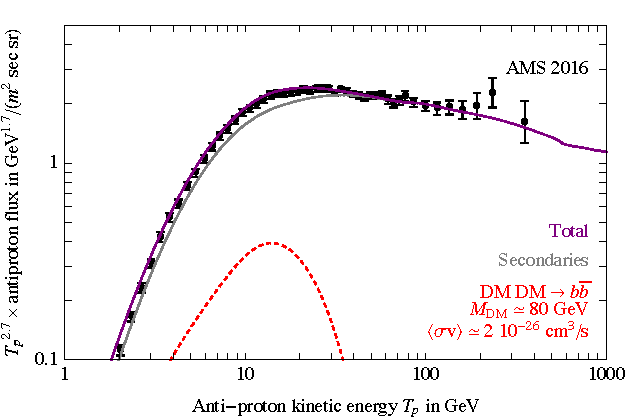
\includegraphics[width=0.48 \textwidth]{figs/CRdata_AMSpbar_excess} \quad
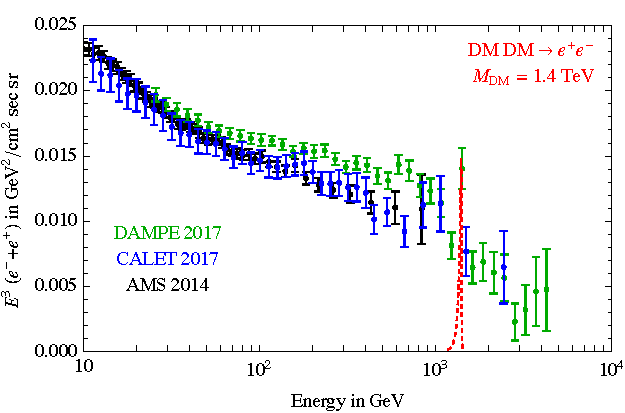
\includegraphics[width=0.48 \textwidth]{figs/CRdata_DAMPE_CALET_2017} 
\end{center}
\caption[Recent claimed excesses in charged cosmic ray data.]{\em\label{fig:pbarandDAMPEexcesses} Illustration of {\bfseries  recent claimed excesses in charged cosmic ray data}. Left: potential antiproton excess in {\sc Ams} data. The grey line represents the astrophysical flux of secondary $\bar p$ that,  together with a DM contribution (red dashed line), would best fits the data according to recent studies. The secondary $\bar p$ best fit flux without DM is not shown. 
Right: possible lepton excess in {\sc Dampe} data.}
\end{figure}



\subsection{An electron+positron {\sc Dampe} excess?}\label{sec:DAMPE}
In 2017 the {\sc Calet}~\cite{Calet} and {\sc Dampe}~\cite{Dampe} experiments released 
their measurements of the `all leptons' spectrum ($e^++e^-$)~\cite{DAMPEepem,CALETepem}, the zoomed in version of which is shown in fig.~\ref{fig:pbarandDAMPEexcesses} (right). 
The {\sc Calet} data are in good agreement with the previous measurements of the same quantity by {\sc Ams}, while the {\sc Dampe} data indicate a higher flux and a harder spectrum. 
The source of this discrepancy remains unclear, 
and could be due to an incorrect energy calibration of one, two or all three of the experiments 
(all three have to rely on extrapolations above $E \approx 100$ GeV, since for such high energies the test beam data are not available). 


While the {\sc Calet} data have remained relatively unexploited, various papers interpreted the {\sc Dampe} data 
in terms of DM~\cite{DAMPEexcess}. Two main features attracted attention: {\em a)} the hint of a spectral break around 0.9 TeV; {\em b)} the single {\sc Dampe} data point at $E \simeq 1.4$ TeV, which formally sits 2.6 $\sigma$ (global) above the power law spectrum prediction. The point a) is not qualitatively different from the knee-like feature discussed in section~\ref{sec:positronexcess}. Fitting b) in terms of DM requires DM annihilating or decaying into $e^+e^-$, inside a very large ($\sim 10^8 \ M_\odot$) and very close clump (within 0.3 kpc). Any other channel and/or a more distant clump (or a smooth DM distribution) would not result in such a sharp spectrum. 





\subsection{The {\sc Anita} anomaly}\label{sec:ANITA}\index{Anomaly!{\sc Anita}}
{\sc Anita}, a balloon-borne radio antenna, has conducted several  one-month-long flights over Antarctica since 2006~\cite{Anita}. It was primarily designed to detect ultra-high-energy neutrinos via the Askaryan radiation which these emit when hitting the ice (the effect can be thought of as a collective \v Cerenkov radiation from the particles in the compact shower initiated by the neutrino). {\sc Anita} was also sensitive to the radio emission of Extensive Air Showers (EASs) produced by ultra-high-energy particles in the atmosphere: either ordinary cosmic rays from the upper atmosphere, or $\tau$ leptons decaying in the air after production in the ice layer by a $\nu_\tau$ that has skimmed the Earth (the focus is on the $\tau$ flavor since electrons and muons are absorbed before emerging from the ice). 


\medskip

{\sc Anita} reported the detection of two puzzling events which appear to be {\it upward}-traveling and very energetic EASs ($\approx$0.6 EeV in both cases)~\cite{ANITAanomaly}. They are puzzling because $\tau$ neutrinos with such extreme energies interact too much with matter and thus cannot traverse the Earth, even taking into account $\tau$-regeneration (see section \ref{sec:DMnuprop}).\footnote{An alternative and more mundane interpretation posits that the signal is the reflection on the ice surface of `ordinary' downward cosmic ray events, not correctly reconstructed by the experiment.}
Since dark sector constructions can include particles that interact with matter less than neutrinos do, various DM-related interpretations have been put forward. In these models, super-heavy DM particles (e.g., with~$M > 10^{10}$ GeV) decay into lighter, extremely boosted particles that are then responsible for the observed signal. 
Other new-physics interpretations, unrelated to DM, have also been proposed, 
based on hypothetical particles that are less interacting than neutrinos, but possibly produced through neutrino conversion.


\medskip

In 2020 {\sc Anita} reported a detection of four additional very high-energy ($\approx$ EeV) events, which are not upward-traveling but rather horizon-skimming~\cite{ANITAanomaly2}. These are not puzzling by themselves, since they can be produced by (unusual but not impossible) very-high-energy $\tau$ neutrinos. However, such a SM explanation is in tension with the limits imposed by other observatories such as {\sc Auger} and {\sc Icecube}. These events have thus also been interpreted in terms of decaying DM with an EeV mass.



\subsection{A Gamma-Ray Burst 221009 anomaly?}\label{sec:GRBanomaly}\index{Anomaly!GRB 221009}
In 2022 two experiments claimed  
the detection of unusually high-energy photons about 1 hour after the
GRB 221009A $\gamma$-ray burst happened at high red-shift $z\approx 0.15$.
{\sc Lhaaso}, in China, claimed an observation of photons up to 18 TeV (later revised to 13 TeV);
{\sc Carpet-2}, situated at Baksan in Russia, claimed an air shower consistent with a 251 TeV photon~\cite{GRBanomaly}.
If the temporal coincidence means that the photons come from the extragalactic $\gamma$-ray burst
rather than from a nearby source, this poses a puzzle: the photon energies are above the threshold for absorption on the extragalactic background light, as discussed in section \ref{sec:cosmogammas}.
That is, the optical depths for  photons originating from $z\approx 0.15$ are $\tau_{\rm opt} \approx 10^4$ at $251\TeV$ and
$\tau_{\rm opt} \approx 14$ at $18\TeV$ (although the uncertain star-light contribution is dominant at this lower energy).
The resulting $e^{-\tau_{\rm opt}}$  suppression of the flux is certainly too large for the 251 TeV photons, and possibly also for the 18 TeV photons.

According to some authors~\cite{GRBanomaly}, the absorption can be avoided or mitigated in the presence of new physics,
such as photon/axion oscillations where the axion has a mass $m_a\sim 10^{-10}\GeV$ and
the coupling to photons is $g_{a\gamma\gamma}\sim 10^{-11}/\GeV$ (axion as a DM candidate is discussed in 
section~\ref{axion}).

\subsection{A 220 PeV neutrino?}\label{sec:220PeVanomaly}\index{Anomaly!220 PeV}
In 2025, the {\sc Km3NeT} collaboration announced the detection of a cosmic-ray neutrino event of apparent extragalactic origin, 
with an estimated energy of approximately  $220 \PeV$~\cite{220PeVanomaly}. 
This energy is an order of magnitude higher than that of neutrinos observed by the similar {\sc IceCube} experiment. 
The event might just be a $\sim 3\sigma$ fluctuation in the observation of neutrinos of astrophysical origin.
However, some authors interpret it as evidence of a spectral hardening in the cosmic-ray neutrino energy distribution, 
potentially due to an additional component arising from the decay of super-heavy DM~\cite{220PeVanomaly}.
The required DM mass would be in the range of hundreds of PeV, with a lifetime around  $10^{29}\,{\rm sec}$,
close to the indirect detection bounds for typical decay channels involving neutrinos (see fig.\fig{IDconstraintsdecay}).




\section{Collider/accelerator: current anomalies}
Several anomalies seen in data from colliders and accelerators admit possible new physics interpretations that could include
DM. Sometimes the connection to DM is direct, for instance the neutron decay anomaly (section \ref{neutrontau}) can be explained by requiring a sizable decay rate to invisible states. In other cases, for instance in the $(g-2)_\mu$ and the $R_{K^*}$ anomalies (sections \ref{sec:g-2} and \ref{sec:RK} respectively), the connection with DM is indirect, with DM possibly contributing through one-loop corrections.  



\subsection{The $(g-2)_\mu$ anomaly}
\label{sec:g-2}\index{Anomaly!muon $g-2$}
The anomalous magnetic moment of the muon, $a_\mu=(g-2)_\mu/2$, 
is a precisely measured quantity with experimental and theoretical errors below the $10^{-6}$ level. 
The measurement by the {\sc Fermilab} Muon $g-2$ Experiment~\cite{muong-2measurements}  confirmed, with improved precision,
the  2006 measurement by the  {\sc Bnl} E821 experiment at Brookhaven~\cite{muong-2measurements}. 
QCD loop corrections to the photon propagator induce
the dominant uncertainty on the theoretical predictions of $a_\mu$.
These effects have been computed in two ways:
\begin{enumerate}
\item Via dispersion relations using $e^+e^-$ scattering data,
with the dominant contribution from $e^+ e^-\to \pi\pi$ close to threshold. 
This technique was adopted for the so-called 2021 {\em consensus} SM prediction \cite{MuonConsensus},
which showed a  $5\sigma$ tension with the experimental results.
The issue is not settled, however, with more recent $e^+e^-$ scattering data from {\sc Cmd}-3 implying no anomaly~\cite{CMD-3}.
\item Via lattice QCD computations. This technique shows agreement with the experiment~\cite{BMW}.
A revised consensus shows no anomaly~\cite{MuonConsensus}.
\end{enumerate}
A  deviation in $\Delta a_\mu$ could have implications for DM models. Both the SM and new physics contributions to $a_\mu$ start at 1-loop. The new physics interpretations can thus include DM running in the loop, if DM has couplings to muons. The models for new physics explanations of $\Delta a_\mu$ fall into two broad categories. In the first category the chirality flip required by $\Delta a_\mu$ is due to the muon mass insertion on the external muon leg. The new physics contribution to $a_\mu$ is thus heavily suppressed by the muon mass, so that the new physics that explains the deviation needs to be light. The most prominent example is a light ${\mathcal O}(100~{\rm MeV})$ gauge boson, for instance due to a new $L_\mu-L_\tau$ gauge group. 


In the other class of models the chirality flip arises from the Higgs coupling to the internal states running in the loop. 
New physics can have a large coupling to the Higgs, and can thereby be
heavy, up to a few TeV, and still explain the $a_\mu$ anomaly.
If the new physics states running  in the loop are odd under some $\mathbb{Z}_2$ symmetry, 
the lightest state is stable, and can be a DM candidate. In fact there are many such DM models that even lead to the right DM thermal relic abundance~\cite{muong-2models}. 

 

\subsection{The flavour anomalies}\label{sec:RK}\index{Anomaly!flavour}
In the period 2014-2022, some deviations from the SM have been claimed in 
rare processes corresponding to the quark level transition $b\to s \mu^+\mu^-$. 
The $b$ and $s$ quarks are bound inside hadrons, so not all observables are theoretically clean, and may involve non-perturbative QCD effects. 
However, the muon-to-electron ratios such as
$R_K =\sfrac{{\rm BR} \left ( B^+ \to K^+ \mu ^+ \mu ^-\right )}{{\rm BR} \left ( B^+ \to K^+ e^+ e^-\right )}$
(and similar for $K_S$, $K^{*+}$) are theoretically clean. 
Away from the kinematical thresholds  such ratios are predicted in the SM to be very close to 1, 
since the electroweak interactions do not distinguish between different lepton generations. 
The only symmetry-breaking effects are due to different muon and electron masses, 
and can be easily taken into account in theoretical predictions. 



The most precise measurements of these quantities are due to the LHCb experiment at CERN,
which originally claimed $R_{K^{(*)}}$ values around $0.8$~\cite{RKanomaly}. 
Global fits to both $R_{K^{(*)}}$ as well as the $b\to s \mu^+\mu^-$ branching ratios and angular distributions in several decay channels then implied 
a statistical significance of the anomaly of about $ 5\sigma$ \cite{RKfits}. 
These anomalies could be fitted by adding to the SM the effective operators of the form
$(\bar s \cdots  b)(\bar\ell \cdots \ell)/(30\TeV)^2$, where the ellipses denote appropriate chiral structures.
The operators could be mediated by new TeV  states, including DM.  In the 2022 analysis the LHCb collaboration improved their treatment of systematic effects in the measurement, which then resulted in revised $R_{K^{(*)}}$ values close to 1, in agreement with the SM. 
The remaining anomalies are now only in the less easily predictable observables affected by the non-perturbative QCD effects.



There is also a hint of anomalies in a different set of theoretically clean ratios, $R_{D^{(*)}}\equiv {\rm BR}(\bar B \to D^{(*)}\tau\bar\nu_\tau)/{\rm BR}(\bar B \to D^{(*)}\ell\bar\nu_\ell)$. However, their statistical significance is less notable. 




\subsection{The neutron decay anomaly}\label{neutrontau}\index{Anomaly!Neutron decay}

\begin{figure}[t]
$$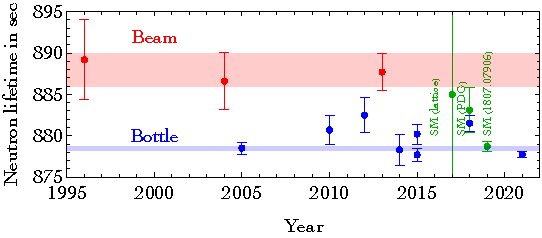
\includegraphics[width=0.7\textwidth]{figs/NeutronAnomalyData}$$
\caption[Neutron decay data]{\label{fig:NeutronAnomalyData} \em
`Bottle' (blue) and `beam' (red) determinations of the {\bfseries neutron lifetime}, compared to the SM prediction (green).}\end{figure}

At low energies, DM has been suggested as a possible explanation of an anomaly in the neutron lifetime measurements.
The neutron undergoes weak $\beta$ decays, where  the
dominant decay channel, 
$n\to p e\bar\nu_e$, already has a highly suppressed decay rate   $\Gamma_n^\beta \sim G_{\rm F}^2 (m_n - m_p)^5$.
The neutron lifetime  is measured using two different experimental techniques,
which consistently give results that differ at about $4\sigma$ level~\cite{NeutronBottleAnomaly},
as summarized in fig.\fig{NeutronAnomalyData}:
\begin{itemize}
\item The {\bf `bottle' method}. 
Ultra-cold neutrons are stored in a magnetic bottle via a small trapping potential, $V_{\rm trap}\approx 50\,{\rm neV}$. 
After some time $t$ the neutrons remaining in the magnetic bottle are counted, fitting the result to $N(t)= N_0 e^{-\Gamma_n^{\rm tot}  t}$. This
 measures the total neutron decay width, giving  $\Gamma_n^{\rm tot} = 1/(879.4\pm 0.6)\s$.
\item The {\bf `beam' method}. A beam of cold neutrons is monitored by counting the protons from 
the neutron $\beta$ decays, 
and fitting the result to $dN/dt = -\Gamma_n^\beta N$.
The measured decay rate, which is here entirely attributed to $\beta$ decays since it is signalled by the counted protons, is found to be smaller,  $\Gamma_n^\beta = 1/(888\pm 2)\s$.
\end{itemize}
The SM predicts $\Gamma_n^{\rm tot} = \Gamma_n^\beta$, up to known additional decay channels, which
 contribute at the $1\%$ level.
The neutron decay anomaly, i.e., the mismatch between  $\Gamma_n^{\rm tot}$ and $\Gamma_n^\beta$, could be due to an entirely new decay channel, where the neutron decays into nearly invisible particles, including DM.
The most discussed possibility is $n\to {\rm DM} \, \gamma$ with $M  \circa{<}  m_n$; 
$n\to 3{\rm DM}$ with $M \circa{<} m_n/3$ is also possible~\cite{NeutronBottleAnomaly}.
Alternatively, for large enough cross sections, the neutrons stored in a bottle could be kicked out by soft scatterings with DM particles, which were captured and thermalized in the Earth~\cite{NeutronBottleAnomaly}. 


\smallskip

The above interpretations are in tension with the precise SM prediction for the neutron decay rate,
 $\Gamma_n^{\rm SM} = 1/(878.7 \pm 0.6)\s$. This agrees with the experimental  `bottle method' result and thus, if correct, leaves no room for the type of new physics contributions that increase the decay rates, 
 indicating a problem with the `beam' measurements.
The caveat is that 
the quoted precise SM prediction employs the determinations of $V_{ud}$ 
and the {\sc Perkeo III} measurement of the neutron axial coupling constant $g_A$~\cite{gAexp},
which are potentially problematic at the claimed level of precision.
The less precise aSPECT~\cite{gAexp} measurement of $g_A$, for instance, favours
the value of  $\Gamma_n^{\rm SM} $ that is close to the beam experiment result.
This additional layer of experimental uncertainty adds confusion to the subject~\cite{NeutronBottleAnomaly}.

\smallskip

An entirely different possibility, which does not run into issues with the $\Gamma_n^{\rm SM}$ problem, is that the neutron decay anomaly is due to a neutron oscillating into a  quasi-degenerate DM state~\cite{NeutronBottleAnomaly}.
A mass splitting between the normal neutron and the DM state of order $\Gamma_n^{\rm tot}-\Gamma_n^\beta$ is needed. 
The DM state then decays invisibly with the same lifetime as the neutron (a possible reason for this would be that DM is a mirror neutron, $n'$, decaying via the $n'\to p' e'\bar\nu_e'$ channel~\cite{MirrorSM}).
The net result is a deficit of protons measured in the beam experiments, while there is no modification of the neutron lifetime when measured using the bottle method.
The above interpretation is consistent with the experimental bounds on the loss of neutrons through the wall of the bottle, 
if the strong magnetic fields $B\approx {\mathcal O}(1) \, {\rm T}$,
used in the beam experiments, enhance oscillations via resonance effects.

\smallskip

All the new physics models need a large coupling between neutron and DM. This implies that DM is produced inside  neutron stars. The resulting equation of state is softened and tends to be incompatible with the existence of heavy neutron stars, which are observed to have masses up to 2 solar masses.\footnote{The physics reason behind it is the same as for the Oppenheimer and Volkoff's calculation in 1939, in which they obtained an {\em underestimated} value for the maximal mass of neutron stars, because they neglected neutron--neutron interactions. The pressure is lowered at a given energy density because DM replaces neutrons and reduces their Fermi momentum and pressure.}
Possible ways out are that the $n\to 3\,{\rm DM}$ decay channel is open (this has a milder effect on the equation of state, and thus remains compatible with data), or that
DM exhibits a strong repulsive force with itself or with neutrons (this makes it expensive to produce DM particles in a purely baryonic medium, both from an energetic point of view and from a chemical potential one)~\cite{NeutronBottleAnomaly}.
In the latter case, the required DM scattering cross section is  comparable with the typical QCD cross sections, and thus risks being in conflict with the bullet-cluster bound on DM interactions, eq.\eq{bulletbound}.



\begin{figure}[t]
$$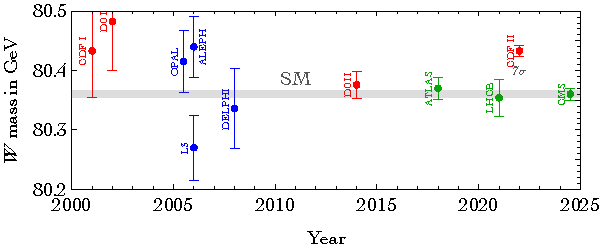
\includegraphics[width=0.7\textwidth]{figs/WmassMeasurments}$$
\caption[$W$-mass data]{\label{fig:WmassMeasurments} \em
{\bfseries  $W$-mass measurements} from LEP (blue), LHC (green), and {\sc TeVatron} (red), compared to the SM prediction (gray) from global electroweak fits.}\end{figure}

\subsection{The $W$-mass anomaly}
\label{sec:CDFWmass}\index{Anomaly!$W$ mass}
In 2022, the CDF TeVatron collaboration reported a measurement of the $W$-boson mass $M_W$ that is $0.7\, \permille$ higher than the SM prediction~\cite{WmassAnomaly}. 
The statistical significance of this tension is $7\sigma$.
The CDF result was also in $\approx 4\sigma$ tension with the other less precise direct experimental determinations of $M_W$.
In 2024 the CMS LHC collaboration reported a measurement of $M_W$ with precision comparable to CDF, but in agreement 
with all the other measurements, and also with the SM prediction.
%The SM predicts $M_W = M_Z \cos\theta_{\rm W}$, plus quantum corrections,
%where the $Z$-boson mass, $M_Z$, and the weak angle, $\theta_W$, 
%have been precisely measured at the $Z$-pole.
The most plausible interpretation is that there is a problem with the CDF result.

Alternatively, the CDM $M_W$
anomaly can be accommodated by extending the SM Lagrangian by a single dimension 6 operator
$\Lag=\Lag_{\rm SM} - (H^\dagger D_\mu H)^2/(6\TeV)^2$.
The extra operator can be mediated at tree level by multi-TeV extra scalars that obtain vacuum expectation values or 
by an extra $Z'$ vector boson coupled to the Higgs, $H$. 
Alternatively, it can arise at one loop level in the presence of
new $\SU(2)_L$ multiplets with weak scale mass, but with the masses of
different multiplet components significantly split by interactions with the Higgs.
This latter kind of new physics is in general significantly constrained by the LHC collider data. 
The collider constraints get relaxed if the decays of the multiplet components involve a neutral invisible particle,
which can play the role of DM~\cite{WmassAnomaly}.

\subsection{The $\gamma\gamma$ peak at 750 GeV and other LHC anomalies}\label{sec:diphoton}\index{Anomaly!LHC}
In 2015, at the beginning of the $\sqrt{s}=13\TeV$ Run2 at the LHC, the data taken by the ATLAS and CMS collaborations
hinted at an excess in the
$pp\to\gamma\gamma$ channel, peaked at an invariant mass of around 750 GeV, and with a local statistical significance of about $4\sigma$~\cite{diphoton}.
This unexpected result sparked a plethora of theoretical speculations and interpretations. 
Given that the new particle would have had a weak-scale mass, it could have mediated interactions with DM, producing the desired DM thermal relic abundance via the freeze-out mechanism. However, the excess did not reappear in the next round of data taking, and was soon dismissed as a statistical fluctuation.

\medskip


At the LHC so many different distributions are measured  that on a statistical basis one expects quite a few anomalies at the few $\sigma$ level. 
Over the course of its operation, numerous such anomalies have indeed been observed, only to subsequently disappear as the integrated luminosity doubled. 
The LHC data hint at:
\begin{itemize}
\item[$\rightsquigarrow$] a $\gamma\gamma$ resonance at 95 GeV
at 152 GeV
and at 680 GeV~\cite{2309.03870};
\item[$\rightsquigarrow$] resonant $t\bar t$ production around 400 GeV~\cite{2309.03870};
\item[$\rightsquigarrow$] di-jet production around 1 TeV and 3 TeV~\cite{2309.03870};
\item[$\rightsquigarrow$] non-resonant excess of $e^-e^+$~\cite{2309.03870};
\item[$\rightsquigarrow$] some distributions of multi-lepton events which seem not to agree well with SM backgrounds~\cite{2309.03870};
\item[$\rightsquigarrow$] events with soft leptons plus missing energy indicate tentative excess that could be interpreted as DM~\cite{2403.14759}.
\end{itemize}
More data can clarify if these are all mere statistical fluctuations.


 
\subsection{The {\sc Atomki} excess at 17 MeV}\label{sec:Atomki}
\index{Anomaly!Atomki}
In 2015, the {\sc Atomki} experiment conducted measurements of the $e^\pm$ particles produced in the decay of
 excited $^8{}{\rm Be}^*$, with $J^P=1^+$, into the $0^+$ ground state.
The {\sc Atomki} team reported a $\approx 7\sigma$ evidence for an excess broadly peaked around $\theta\sim 135^\circ$,
where $\theta$ is the angle between the outgoing $e^-$ and $e^+$ (their energies and charges were not measured)~\cite{Atomki}.
The excess can be interpreted as an on-shell production of a new boson $X$ with mass
$(17\pm0.3)\MeV$ and
\beq {\rm BR}(^8{}{\rm Be}^*\to X \, {}^8{}{\rm Be} \to e^- e^+\, {}^8{}{\rm Be})\approx 0.6~10^{-5}\,
{\rm BR}(^8{}{\rm Be}^*\to \gamma \, {}^8{}{\rm Be}).\eeq
Subsequently, in 2021 and 2022, the {\sc Atomki} team identified a similar anomaly at roughly the same mass in the decays of $^4{\rm He}^*$ and $^{12}{\rm C}^*$, respectively~\cite{Atomki}. 
In 2023 a consistent result was obtained by a combined team of {\sc Atomki} and Vietnamese researchers (\href{https://indico.cern.ch/event/1258038/contributions/5538280/attachments/2700698/4687589/X17\%20HUS\%20ISMD2023.pdf}{Ahn (2023)} in~\cite{Atomki}).
Furthermore, the $\gamma\gamma$ resonances at 17 and 38 MeV were reported by \arxivref{2311.18632}{Abraamyan et al.~(2023)}~\cite{Atomki}.
The MEG-II experiment at PSI did not see a signal, disfavouring the ATOMKI claim at $2\sigma$~\cite{2411.07994}.
Improved independent tests are expected soon. 

\medskip

The state $X$  has been tentatively interpreted as a new physics particle: either
a new axion-like pseudo-scalar or an axial vector, coupling to nucleons via a gauge coupling $g\approx 10^{-4}$.
The $X e\bar e$ coupling is less constrained, since in this context only the branching ratio ${\rm BR}(X\to e^-e^+)$ is relevant.
The 2025 results of the $e^-e^+\to X\to e^- e^+$ {\sc Padme} experiment show a tentative $\lesssim 2\sigma$ peak at 17 keV, which at present can
neither confirm nor exclude the ATOMKI anomaly~\cite{PADME}.
Such $X$ could also serve as a mediator between the SM and DM~\cite{Atomki}.
The axial vector (unlike the vector) can simultaneously fit the three {\sc Atomki} anomalies, in Be, C and He.
The pseudo-scalar does not couple to $^{12}{\rm C}^*$, and thus cannot explain that particular excess
(unless parity is broken).
Other bounds can be satisfied but restrict specific combinations of $X$ couplings 
to $p$ and $n$ to suspiciously small values:
$\pi^0\to X\gamma$ bounds force a vector $X$ to be proto-phobic,
 $\pi^+\to e^+ \nu_e X$ bound restrict a pseudo-scalar $X$.

For the {\sc Atomki} anomaly in He several potential explanations within the SM have been put forward as well:
that it is a signal of a light tetraquark state; that it is due to higher order effects; or due to a $^4{\rm He}$ resonance 
with exotic color arrangement in the form of a heavy $(ud)^6$ `hexadiquark'~\cite{Atomki}.
These suggestions, however, still need to be validated by calculations from first principles.


\section{Cosmology: current anomalies}\label{sec:cosmoanomaly}
Global analyses fitting cosmological observations to the $\Lambda$CDM model have highlighted potential discrepancies, which might stem from systematic issues.
Given the significant role that DM plays in cosmology (see section~\ref{sec:evidencesmaxi}), 
various tentative interpretations involve DM, as reviewed below.




\subsection{The cosmic calibration Hubble tension}\label{sec:HubbleTension}\index{Anomaly!Hubble}

\begin{figure}[t]
$$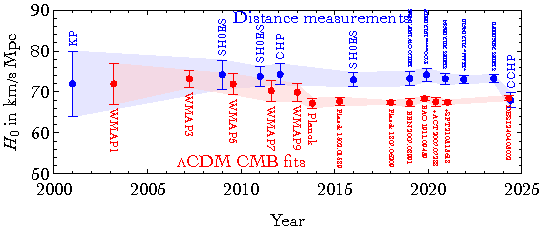
\includegraphics[width=0.69\textwidth]{figs/HubbleAnomalyHistory}$$
\caption[$W$-mass data]{\label{fig:HubbleAnomalyHistory} \em
Time series of determinations of the {\bfseries Hubble constant $H_0$}, either from global $\Lambda$CDM  fits to CMB and structure-formation data (red), or from measurements that use the distance ladders (blue).}
 \end{figure}

Global $\Lambda$CDM fits, in particular the CMB data from {\sc Planck} and at large $\ell \circa{>}1000$, 
prefer a present day  Hubble constant that is lower than what is measured locally, using cepheids and supernov\ae{} Ia, see fig.\fig{HubbleAnomalyHistory}.
The benchmark determinations in the two cases come, respectively, from {\sc Planck}, which finds $H_0 = (67.27\pm 0.6) \,{\rm km/s/Mpc}$, and from the {\sc Sh0es} collaboration, which finds $H_0 = (73.04\pm 1.04) \,{\rm km/s/Mpc}$.
More generally, the tension is between the values of $H_0$ determined by the `early Universe' methods (mainly the CMB, but also BBN and BAO) and the `late Universe' techniques, using supernov\ae{}, the tip of the red giant branch, masers, time delays in strong gravitational lensing (the {\sc H0liCow} project), gravitational wave emitters as standard sirens, and a host of other techniques.
2024 results from the Chicago Carnegie Hubble Program (CCHP) fall however in the middle~\cite{H0tension}.
The magnitude of the tension ranges between $3-6\sigma$, depending on how the systematics of the different probes are evaluated and how different measurements are combined. This so called {\em `Hubble tension'} is one of the most intensely debated issues in cosmology since about 2016~\cite{H0tension}. 


\medskip

Significant modifications of cosmology, usually around or before matter/radiation equality and involving unconventional ingredients, are needed to substantially improve the global fit. 
The first large class of models involves modifying the relative density ($\Omega_{\rm DE})$ or the equation of state ($w_{\rm DE}$) of dark energy, because these are degenerate with $H_0$ as inferred from the CMB. The second class of models makes use of the degeneracy between the number of relativistic degrees of freedom, $N_{\rm eff}$, and $H_0$: one can increase the `early' value of the Hubble constant and bring it closer to the `late' one by introducing extra radiation, such as light sterile neutrinos, axions or other light or massless particles.

\smallskip

In this context, DM can play an important role in several different ways~\cite{H0tensionandDM}. We first review the possibilities within the second class of models introduced above, those in which extra relativistic states are introduced. First, DM can be the origin of the extra radiation: many models have been constructed where (a fraction of) DM is either relativistic or
decays into light relativistic degrees of freedom. DM could decay into neutrinos, into photons, into invisible relativistic particles, or into dark mediators that then decay into radiation. DM can also be in the form of PBHs (section \ref{sec:PBHs}) which, if evaporating at the right time, inject relativistic particles into the thermal bath.
Second, DM can elastically scatter with neutrinos, photons, baryons or with some of the dark radiation particles, thereby effectively acquiring (in small part) the behaviour of extra radiation.
Third, annihilating DM can inject energy into the thermal bath, thereby keeping higher the fraction of the total energy that is in radiation.
 This is the case, for instance, in the cannibal DM scenario (section \ref{cannibalism}), where 3 $\to$ 2 processes effectively convert the energy stored in the mass of the eaten particles into thermal energy of the surviving ones.


In the other class of models, where the Hubble tension is alleviated by modifying the properties of dark energy, DM can still play a role through its coupling to DE. This is realized via an effective mechanism that links non-gravitationally the DM and DE energy densities in the cosmological Boltzmann equations (see section \ref{sec:CMB}). As a result, at specific epochs some of the DM energy density is converted into DE (or vice versa), modifying the cosmological history and therefore the determination of the Hubble constant. 
There are numerous concrete implementations of this mechanism.
 Alternatively, there are models in which DM and DE are assumed to be a single fluid, which behaves as DM at early times and as DE at late times. The evolution of the Hubble rate with redshift is therefore modified and this allows to alleviate the tension. 

\smallskip

As of this writing it seems that some of the models involving DM can only partially reduce the $H_0$ tension, 
and that obtaining a convincing solution is not easy. 
The situation is further complicated by other milder anomalies,  
%such as the $S_8$ anomaly discussed next in section~\ref{sec:S8}, 
as well as by internal tensions, e.g.,\ in Planck data, 
and tensions between different experiments.
The situation may well imply that 
 presently the uncertainties are underestimated, though many experimental checks have been performed. 



\subsection{The matter inhomogeneity $S_8$ anomaly}\label{sec:S8}
The amount of matter inhomogeneities in the low-redshift Universe $z\circa{<}1$ is quantified by the $S_8 = \sigma_8(\Omega_{\rm m}/0.3)^{1/2}$ parameter, where $\sigma_8$ is (roughly speaking) the amplitude of the matter power spectrum smoothed over scales of 8 Mpc$/h$. 

Several local determinations of $S_8$ performed over the years, e.g.~using weak lensing, galaxy clusters and other techniques, had consistently found a value about $3\sigma$ lower than the predictions of global $\Lambda$CDM fits. In other words, the clustering of matter observed in the late Universe seemed smoother than what it would be expected based on the evolution of the early anisotropies (matter clustering at higher redshift, instead, agreed with $\Lambda$CDM). This is the so-called `$S_8$ anomaly'. 
The situation evolved in 2024 and 2025, when new local determinations, notably by the Kilo-Degree Survey ({\sc KiDS}) using cosmic shear but also by {\sc Act} and {\sc Spt} using CMB lensing (see section \ref{sec:bullet}), found a value $S_8 \approx 0.82$ in agreement with the global fits~\cite{S8anomaly}.

\smallskip

Various authors had tried fitting the $S_8$ anomaly by assuming new physics that slows down the clustering of matter without conflicting with other observables~\cite{S8anomaly}.
For instance, by assuming that cold DM decays into warm DM and dark radiation with a lifetime $\tau\approx{\rm Gyr}$,
or by assuming that DM undergoes DM DM $\leftrightarrow$ DM DM DM scatterings,
or that DM interacts with Dark Energy (which is a somewhat natural guess since the anomaly corresponds to the era in which DE starts to dominate over DM).\index{DE-DM interaction}


\subsection{The {\sc Desi} anomaly}\label{sec:DESIanomaly}
Various experiments measure the late expansion history of the Universe, at scale factor $a \gtrsim 0.1$,
by relying on different probes: supernov\ae{} Ia as standard candles,
baryon acoustic oscillations as a standard size in matter inhomogeneities, and the CMB.
These measurements of $H(a)$ are often presented as
$w_{\rm DE}(a)$, given that the late-time Universe is dominated by Dark Energy
and that DE might exhibit an unusual equation of state (we remind that the latter is defined as $p_{\rm DE}=w_{\rm DE}\rho_{\rm DE}$, resulting in $d\ln\rho_{\rm DE}/d\ln a = -3 (1+w_{\rm DE})$, see Appendix \ref{app:matterenergy}).

The $\Lambda$CDM model assumes a cosmological constant, i.e. a constant $\rho_{\rm DE}$, and thus $w_{\rm DE} \equiv-1$.
Data from the {\sc Desi} collaboration, however, indicate a $\approx 3\sigma$ hint for a deviation from $\Lambda$CDM, suggesting that
$w_{\rm DE}$ increases with time, being $w_{\rm DE} \approx -0.7$ now and $w_{\rm DE}<-1$ at $a\sim 0.5$~\cite{DESIanomaly}.
This is puzzling, since $w_{\rm DE} <-1 $ means that $\rho_{\rm DE}$ grows with time.
A possible way of reconciling a growing $\rho_{\rm DE}$ with basic principles of physics is that DE
interacts with some other component, receiving energy from it.
DM is a natural candidate, given that it is the second dominant component in the energy budget of the Universe, while its interaction properties are not known. 

\index{DE-DM interaction}
A possible theory is that DE is the vacuum energy of some very light scalar field $\phi$ that controls the mass of DM particles $M(\phi)$~\cite{DE2DM}.
For example DM might be a fermion with a Yukawa coupling to $\phi$.
As the DE scalar evolves in the effective potential $V_{\rm eff}=V(\phi) + \rho_{\rm DM}$, 
 the DM density $\rho_{\rm DM} \propto m(\phi(a))/a^3$ can also change,  and thus the DM equation of state is also modified.
This physics can be presented by including the anomalous variation of DM density in an effective DE energy density
\beq 
\rho_{\rm DE}^{\rm eff} = \rho_{\rm DE} + \rho_{\rm DM} [1 - M(\phi_0)/M(\phi)],\qquad\Rightarrow\qquad
w_{\rm DE}^{\rm eff} = \frac{w_{\rm DE}}{1+(\rho_{\rm DM}/\rho_{\rm DE})[1-M(\phi_0)/M(\phi)]},
\eeq
while the effective DM density is the  one that would follow from a constant DM mass, $\rho_{\rm DM} [M(\phi_0)/M(\phi)]$.  A DM mass that increases with time can thus mimic a DE with equation of state 
%$w_{\rm DE}^{\rm eff}  < w_{\rm DE} \le -1$.
%\\
$w_{\rm DE}^{\rm eff}  \leq -1$.

In a variation of the same idea, DM is an oscillating axion-like field $a$ with kinetic term $K(\phi)(\partial_\mu a)^2/2$ that depends on $\phi$, that thereby again induces a variation of the axion mass $m_a$~\cite{DE2DM}.



 
\subsection{The dipole anomaly}\label{sec:dipoleanomaly}
The large observed CMB dipole is interpreted to be due to our local motion with
\beq |\mb{v}_{\rm sun} | \approx 370\,{\rm km/s}\qquad \hbox{and}\qquad
 |\mb{v}_{\rm local~group} | \approx 620\,{\rm km/s},
 \eeq
relative to the CMB rest frame. 
According to standard cosmology, this should also be our velocity with respect to distant matter, at red-shifts $z\circa{>} 1$.
The same dipole in the observed sky brightness should thus also be seen with astrophysical probes. However, some (but not all, see \arxivref{2205.06880}{J.~Darling} in~\cite{dipoleanomaly}) 
surveys find a velocity that is a factor of a few larger, in roughly the same direction~\cite{dipoleanomaly}, where one should keep in mind that 
these astrophysical measurements of the dipole are more difficult than the measurement of the CMB dipole.
If confirmed, this would challenge the view that matter is  nearly homogeneously distributed on large scales.
Standard cosmology would then need a drastic revision, with implications for DM.


\subsection{The {\sc Edges} 21 cm anomaly} \label{sec:EDGESanomaly}\index{Anomaly!21 cm}
In 2018, the Experiment to Detect the Global Epoch of reionization Signature ({\sc Edges}) reported an observation of the signature corresponding to the absorption of 21cm radiation by cosmic neutral hydrogen at redshift $z\approx 17$. The amount of absorption, in its simplest interpretation, implied that the temperature of the neutral gas at that epoch was significantly lower than what is expected in the standard $\Lambda$CDM cosmology, with a statistical significance of about $3.8\sigma$~\cite{EDGESexp}. 

\smallskip

This was surprising given that the thermal history of cosmic hydrogen, while rather complex, is well understood within the standard cosmology.\footnote{The broad formalism for the evolution of the gas temperature has already been sketched in section \ref{sec:boundsTigm}.} It is worth reviewing qualitatively the main phases of the evolution in order to better understand the possible origins of the anomaly. 
Before recombination, the photon and the gas fluids had the same temperature. At the moment of recombination ($z \sim 1100$, i.e., when the Universe was 380 kyr old), the photons, which from that moment constitute the CMB, and the newly formed neutral hydrogen atoms scattered for the last time. However, the residual Compton interactions kept the two fluids thermally coupled for much longer, until approximately $z \sim 150$ (or 8 Myr). Subsequently, the gas, also referred to as the intergalactic medium (IGM),  thermally decoupled from the CMB and began cooling adiabatically as $T_{\rm igm} \propto (1+z)^2$. This is faster than the cooling of CMB, whose temperature scales as $T_{\rm CMB} \propto (1+z)$. 
 As a result, $T_{\rm igm}(z)$ became lower than $T_{\rm CMB}(z)$, starting from their common value at $z \sim 150$. This remained true at least until the era of cosmic dawn, when the first stars started emitting light, 
 eventually raising the gas temperature above that of the CMB at $z\circa{<} 15$.
Distinct from $T_{\rm igm}$, the hydrogen `spin temperature' $T_S$ is defined by $n_1/n_0 \equiv 3 e^{-\Delta E/T_S}$ and parameterizes the relative population of the two ground state levels of cosmic neutral hydrogen, with spin $S=0$ or $S=1$ and the energy difference $\Delta E = 2\pi/(21 \cm)$. During the dark ages ($z \sim 1100 \to 20$) and through cosmic dawn ($z \sim 20 \to 15$), $T_S$ evolved between the `floor' value $T_{\rm igm}$ and the `ceiling' value $T_{\rm CMB}$. 
Whenever $T_S < T_{\rm CMB}$, the background CMB photons shining on the clouds of cold hydrogen gas get absorbed, generating a dip in the spectrum. 
This is notably the case around $z \approx 17$ leading to the expectation that CMB photons that had a wavelength of 21 cm at that time, corresponding to 70-80 MHz today, i.e.,\ the very low-energy portion of the CMB, should be missing from the measured spectrum of the CMB. By analyzing the depth of this absorption dip, one can obtain information about the temperature of the gas and the CMB at that epoch. 
This dip in the CMB spectrum is exactly what {\sc Edges} measured. 


More precisely, the experiment measured the quantity $T_{21} (z) \approx  23 \,   \mathrm{mK} \left(1 - \sfrac{T_{\rm CMB}(z)}{T_{S}(z)} \right)$, which expresses the difference between the brightness temperature of the 21 cm hydrogen emission and the temperature of the low-energy portion of the CMB radiation.  
{\sc Edges} found $T_{21} \approx -0.5^{+0.2}_{-0.5} \, \mathrm{K} $ at 99\% C.L., while standard astrophysics predicts $T_{21}\approx -0.2\,{\rm K}$ at $z\approx 17$. Qualitatively, this means that the difference between the floor ($T_{\rm igm}$) and the ceiling ($T_{\rm CMB}$), between which $T_S$ can evolve, is larger than expected.

\smallskip


The {\sc Edges} measurement  required a careful subtraction of an overwhelmingly intense foreground, approximately $10^4$ times stronger than the signal under investigation. 
Assuming that the net result is correct, the detected anomalous temperature difference requires physics beyond the Standard Model. There are two ways to solve the discrepancy with new physics. On one hand, one can `lower the floor', i.e.,~cool the hydrogen gas more efficiently than in the standard cosmology. On the other hand, one can `raise the ceiling', i.e.,~increase the temperature of the CMB photons. 


\medskip

DM can potentially play a pivotal role in both of these scenarios~\cite{EDGES}. On one side, since DM decoupled much earlier than the gas, the DM fluid is much colder than hydrogen during the dark ages, including at $z \approx 17$. 
Prompted by the {\sc Edges} measurement, it was thus quickly suggested that DM-baryon scatterings could offer an efficient mechanism to cool down the hydrogen gas. 
 These scatterings might also occur between baryons and a fraction of DM, possibly with DM being milli-charged. 
On the other hand, additional 21-cm radiation could be injected via the decays or annihilations of DM particles, from the evaporation of Primordial BH DM, or via the conversion of axion-like DM into photons. This would effectively heat the CMB spectrum. Observationally this is not a problem, since the CMB is poorly measured in its very low-energy portion.


The {\sc EDGES} results can be approached from a different angle:
one can give up on trying to explain the discrepancy, and simply focus on the fact that an absorption feature has been detected. This implies that the gas was colder than the CMB at $z \approx 17$, which then imposes stringent bounds on DM annihilations or decays that would have heat the gas \cite{EDGESbounds}. 

\medskip


Future experiments such as {\sc Lofar}, {\sc Saras}, {\sc Bighorns}, {\sc Leda}, {\sc Mwa}, {\sc Assassin} or {\sc Ska} \cite{EDGESexp} will test the absorption signal and may shed light on the potential involvement of DM. 
Preliminary results from the {\sc Saras3} experiment  (\arxivref{1710.01101}{Singh et al.~(2022)} in~\cite{EDGESexp}) do not confirm the {\sc Edges} findings.




\setlength\epigraphwidth{0.67\textwidth}

\section{Astrophysics: current anomalies}
\label{sec:astroanomaly}
\label{CDMproblems} 

An astrophysical anomaly may sound like an oxymoron,\footnote{ ``{\em A single hydrogen atom in conflict with quantum mechanics would be a tragedy. A single galaxy in conflict with {\rm $\Lambda$CDM} can be an outlier}'' ($\sim$ M. Bauer).} given that in astrophysics one cannot perform repeatable experiments, but rather only make observations, contrary to fundamental physics that can be done in a laboratory. Taking into account this limitation, we summarize below possible issues discussed in the literature.

\medskip

First, we discuss various puzzling features related to the DM density distribution on galactic (section \ref{sec:cuspcore}) and sub-galactic (section \ref{sec:missingsatellite}) scales. These are also referred to, rather dramatically, as the `small scale crisis' \cite{DM:density:anomalies}. 
It is worth noticing that these features often point to a disagreement between numerical simulations (see section~\ref{Nbody}) and observations, i.e.,~they  point to our still limited understanding of what DM is and how it behaves. This is contrary to most of the other anomalies discussed in the other sections of this chapter, which instead are deviations from known physics and thus hint at DM.
Then, we discuss the black hole mass gap (section \ref{sec:BHmassgap}) and stochastic gravitational waves (section \ref{sec:NANOgrav}).

\index{DM problems!cusp-core}\index{DM problems!diversity}
\subsection{Galactic-scale anomalies} \label{sec:cuspcore}
\index{Numerical simulations!cusp-core problem}

\begin{itemize}
\item[$\blacktriangleright$] The ``{\bf cusp-core problem}'' \cite{corecusp}. Numerical $N$-body simulations that include only collision-less cold DM and gravity predict DM halo density profiles that for $r\to 0$ grow as $1/r^\gamma$, $\gamma\approx 1 -1.5$, giving a cusp in the galactic center. Observations, however, tend to favour constant density cores, see section \ref{rho(r)}. 
Various authors speculated that this so called {\em cusp-core problem}\footnote{From rotation curves it is easier to measure the total mass up to a certain radius in the inner region, while its derivative, i.e., the DM density profile, is harder to determine. The problem is thus more robustly phrased as the {\em ``inner mass deficit''}: DM only simulations predict more DM in the inner regions of galaxies than what is observed.} points to a more complex DM.
Cored profiles can, for instance, arise if DM is ultralight (fuzzy DM, section~\ref{LightBosonDM}), with the de Broglie wavelength comparable to the size of the DM halo core. Another possibility is that DM is self-interacting (section~\ref{sec:SIDM}), in which case the interactions affect the evolution of DM halos. Initially, warm DM (section~\ref{sec:WarmDM}) was also invoked as a possible solution, but this tends to run afoul of other observations, which bound the DM mass to be above few keV, so that DM needs to be effectively cold as far as the cusp-core problem is concerned. 

The inclusion of baryons in the $N$-body simulations at least partially resolves the cusp-core problem. 
Actually, early simulations that included baryons showed the opposite effect, where the inclusion of baryons made the cusp-core problem worse since baryons can pull more DM into the centre as the gas cools and condenses, in the so called {\em adiabatic contraction}\index{Adiabatic contraction} process (see, e.g.,~\arxivref{1108.5736}{Gnedin et al.~(2011)} \cite{corecusp}). This was later shown to be due to a too coarse spatial resolution in the early simulations. 
Some early simulations also indicated that the formation of a central bar in the galaxies could turn a cusp into a  relatively large core within a few orbital times. This was later shown to be due to too simplified numerical assumptions.
The situation changed around 2013 when hydro-dynamical simulations became more refined. In particular, the works of 
\arxivref{1306.0898}{Di Cintio et al.~(2014)}, \arxivref{1507.03590}{Tollet et al.~(2016)}, \arxivref{1508.04143}{Read et al.~(2016)} and \arxivref{1605.05971}{Katz et al.~(2016)} in \cite{corecusp} 
showed that whether or not a cusp forms at the center of a simulated galaxy  depends on the stellar-to-halo mass ratio, and can also be a function of time. In the formation of galaxies with few stars, the injection of energy from the stellar feedback is insufficient to significantly modify the inner density of the DM halo. Such galaxies therefore retain the cuspy profile which is typical of DM-only simulations. 
At higher stellar-to-halo mass ratios ($\mathcal{O}(10^{-3}-10^{-2})$), the stellar activity (in particular the supernovae explosions) `pushes out' DM, which makes the gravitational potential shallower and therefore drives the creation of a cored profile. 
At even higher stellar-to-halo mass ratios ($\gtrsim {\rm few} \ 10^{-2}$), the abundance of stars at the center of the galaxy  instead deepens the gravitational potential, recreating a cuspy profile.
The stellar-to-halo mass ratio can evolve with time. The inner density profile of a galaxy can thus change substantially as the galaxy grows in both the stellar and total mass.
In the case of the Milky Way, adopting the estimates given in section \ref{sec:MilkyWay}, the stellar-to-halo mass ratio is quite high ($\approx 0.08$) and thus points towards a cusped inner profile.\footnote{As a word of caution, we mention, however, that the studies quoted above  in \cite{corecusp} draw their conclusions using galaxies somewhat smaller than the MW, and that the slope of the DM density is measured within a rather restricted range of distances from the center, typically $1-2 \%$ of the virial radius.}


\item[$\blacktriangleright$]
 The  ``{\bf diversity problem}'' \cite{diversity}. 
Spiral galaxies with the same maximal circular velocity show larger spread in their interiors and their core densities (\arxivref{0912.3518}{Kuzio et al.~(2009)} and \arxivref{1504.01437}{Oman et al.~(2015)} in \cite{diversity})
than what is expected from the cold DM $N$-body simulations (\arxivref{astro-ph/9611107}{Navarro et al.~(1996)} and \arxivref{astro-ph/9908159}{Bullock et al.~(1999)} in \cite{diversity}).
While for the simulated galaxies the shape of the rotation curves varies as a function of galactic mass, there is little variation between different simulated galaxies that have  the same maximal circular velocity. 
That is, in numerical simulations two galaxies with similar halo masses will have comparable total stellar mass, mass concentration and rotation curves, while observations show a diverse range for these quantities.

The possible resolutions are the same as for the cusp-core problem: (i) DM dynamics could be more complex, (ii) current simulations  may fail to reproduce correctly the effect of baryons, or (iii) the observational determination of mass profiles in the inner parts of the galaxies could be incorrect. However, at present it is far from clear which of these resolutions is the correct one.

\item[$\blacktriangleright$] \label{dynamicalfrictionproblem}
The problem of {\bf DM dynamical friction} \cite{problemdynfriction}.\index{DM problems!dynamical friction}
As discussed in section~\ref{sec:DynamicalFriction},
the gravitational pull from DM produces a frictional force on celestial bodies moving through regions with high DM density.
Several studies, however, suggest that certain astrophysical systems do not exhibit this effect.
For example, some studies have argued that the central bars, present in many of the observed disc galaxies, should have experienced more slowing down from the DM halo friction than what is observed. Similarly, it was argued that the globular clusters in the Fornax dwarf galaxy should have sunk in the center more rapidly than what the observations indicate (this is the so called {\em timing problem}: 
why are at least five of these clusters observed at significant distances from the center of Fornax, if they should have gravitated inward long ago?).
This has been used to argue {\em against} the very existence of DM halos
(see, e.g.,~\arxivref{2106.10304}{M. Roshan et al.}~\cite{DynamicalFriction}), 
or at the very least as an evidence for significant tension with the predictions of the $\Lambda$CDM model. 

However, more mundane astrophysical explanations do exist. 
Some simulations suggest that rotating bars within DM halos can persist, if the bars formed late in the galaxy's history, potentially through a merging event. 
Additionally, certain studies find that a cored DM distribution in Fornax could prevent the inward migration of globular clusters, a phenomenon referred to as \emph{core stalling}~\cite{DynamicalFriction}. 

\item[$\blacktriangleright$]
The {\bf baryonic Tully-Fisher relation}~\cite{Tully-Fisher} is an experimentally observed relation between  the amount of baryonic matter in the galaxy and the maximal rotational velocity in the galaxy (measuring the total amount of DM and visible mass in the galaxy). 

While such a relation between baryon content of galaxies and their halo masses is believed to  arise naturally from galaxy formation, it is currently still hard to tell whether the theoretical predictions from $\Lambda$CDM agree with observations in detail. For further discussion of this issue, see section \ref{sec:Tully-Fisher}. 


\item[$\blacktriangleright$]
%\subsection{The early galaxies anomaly}\label{sec:earlygal}
Starting from 2022, the James Webb Space Telescope ({\sc Jwst}) observed {\bf early galaxies} at redshift $z\gtrsim 7$. These early galaxies are seemingly too massive to be present
in such an early cosmological epoch, at least according to the standard $\Lambda$CDM cosmology, complemented by astrophysical models of star formation ~\cite{JWSTearlygal}.
Various more efficient astrophysical star formation processes could explain such observations.
%If JSWT measurements turn out to truly be anomalous, they 
Alternatively, observations might point to new DM physics, such as a higher DM power spectrum at the relevant scales.
Some authors instead interpret this possible anomaly as evidence for the MOND alternative to DM~\cite{JWSTearlygal} (to be discussed in chapter~\ref{sec:MOND}).


\end{itemize}



\subsection{Subgalactic-scale anomalies}\label{sec:missingsatellite}\index{DM problems!missing satellites}\index{Numerical simulations!missing satellites}

\begin{itemize}
\item[$\blacktriangleright$]
The {\bf missing satellite problem}~\cite{missingsatellite}. The DM-only $N$-body simulations predict many more DM sub-halos (`satellites') than the observed number of  `classical' dwarf galaxies, known prior to the improved searches that started in mid 2000s (see section \ref{sec:dwarfs}). This discrepancy was dubbed the {\em missing satellite problem}, and is now largely resolved. 

First of all, many more new faint satellites were discovered in the Milky Way and Andromeda (M31) galaxies. Furthermore, the $N$-body simulations have improved: they have a better resolution, they include baryons and they can now resolve previously neglected processes such as the fact that the central galaxy potential destroys subhalos on orbits with small pericentres. As a result, the state-of-the art $\Lambda$CDM hydrodynamical numerical simulations are now essentially consistent with the observed number of satellite galaxies, at least once the corrections for the detection efficiencies of the surveys are included. In summary, simulations and observations met mid-way: satellites form in lower numbers then initially predicted, but many are too dark to be seen.


\item[$\blacktriangleright$]\index{DM problems!too big to fail} 
{\bf ``Too big to fail''}~\cite{toobigtofail}. The most massive observed satellites of the Milky Way are smaller than the most massive subhalos obtained in DM-only $N$-body simulations.\footnote{The same discrepancy is found also for Andromeda (M31) and other nearby galaxies.} The question therefore arises: if the Milky Way is supposed to have very massive satellites, where are they and why don't we see them? One possibility would be that such very massive satellites simply do not contain stars, are thus completely dark, and have not been observed. This would be very surprising since such subhalos are massive enough that their gas should have cooled and formed stars, like it did in the smaller subhalos. In other words, the very massive subhalos are {\em ``too big to fail'' (forming stars)}. 

A more likely resolution therefore lies elsewhere. One option is that the total mass of the Milky Way halo is overestimated --- if the mass of Milky Way is in the lower part of the currently allowed observational range (see eq.~(\ref{eq:M200:value})) this would imply that the most massive satellites are also expected to be lighter, in line with observations. The other possibility is simply statistics - there is large halo-to-halo scatter for the mass of the most massive subhalos, and Milky Way could just happen to be one of the downward fluctuations. The too big to fail problem is also less of an issue when comparing with $N$-body simulations that include baryons, in particular because in that case the galaxies can form DM cores instead of cuspy profiles (see section \ref{sec:cuspcore}), and thus lead to smaller halo masses. In summary, there appears to be consensus among current cosmological simulations that there is no `too big to fail' problem for Milky Way and M31 satellites anymore, while it may still be present for isolated dwarf galaxies in the nearby Universe.


\item[$\blacktriangleright$]\index{DM problems!planes of satellites}
{\bf Planes of satellites}~\cite{satellite_plane}. A large fraction of the Milky Way satellites lie in a thin planar disk almost perpendicular to the galactic disk, which appears to be corotating. Something similar is also observed for around half of the satellites of the Andromeda galaxy M31. And some nearby galaxies also show such planar distributions of satellites. This has been one of the more persistent discrepancies between simulations and observations, since simulations predict satellites to be distributed roughly isotropically (spherically or at most slightly prolate), and to possess random motions.

The resolution is not clear, though several possibilities have been discussed:\footnote{The trivial possibility that this is due to a selection bias, i.e.,~only the satellites sticking out of the disk are seen, can be quickly dismissed: the galactic disk of the Milky Way only obscures two relatively thin wedges of about 24 degrees, and outer galaxies are observed even more clearly.} (i) that the presence of massive satellites, such as the large Magellanic cloud, boosts the planarity of the satellite distribution (this is seen in the simulations); (ii) it is possible that the surrounding larger scale cosmological structure needs to be included in the simulations (this is hinted at by the fact that the planar structures of dwarf galaxies in the whole local group of galaxies shows some degree of alignment; by the way, this is claimed to work also in modified Newtonian dynamics, without DM, see \arxivref{1712.04938}{B\'\i{}lek et al.~(2017)}~\cite{satellite_plane}); (iii) the observed alignment could also be just temporary, a situation that appears to be quite likely in simulations (plane configurations are found to last $\sim$ 500 Myr).

\item[$\blacktriangleright$]\index{DM problems!quiescent fractions}
{\bf Quiescent fractions} \cite{quiescentfraction}. Nearly all observed isolated (non-satellite) dwarf galaxies are star-forming, while nearly all satellites of the Milky Way and M31 are {\em quiescent}, with no gas and no star formation. This seems to be in contrast to other Milky Way like galaxies in our local group, for which nearly all their satellites are also star-forming. 

The resolution likely has little to do with DM properties. However, it does raise the following question: if the Milky Way and M31 are outliers in this respect, how representatives are their other properties of an average galaxy, which is what simulations aim to reproduce?

\end{itemize}







\subsection{Black hole mass gaps} 
\label{sec:BHmassgap}
In 2019, the {\sc Advanced Ligo} and {\sc Virgo} collaborations detected a gravitational wave signal from a merger of two black holes, with masses $\approx 66 \, M_\odot$ and $\approx 85 \, M_\odot$ (later revised to slightly higher values). There is about $3\sigma$ probability that at least one of the two BHs lies in the so-called `BH upper mass gap' or the `pair-instability gap', i.e., in the range $ 50 \, M_\odot \lesssim M\lesssim 120 \, M_\odot$. Subsequent results by the {\sc Ligo-Virgo-Kagra} collaboration added a few more candidates with similar characteristics~\cite{LIGO:massive:BH}. 


These results are puzzling --- normal stellar evolution predicts that there should be no BHs with masses in this range, if they were produced from the collapse of a star, due to the following considerations. In the cores of stars  with masses $\gtrsim 50 M_\odot$ the density and temperature is high enough that electron-positron pairs can be efficiently produced from the plasma, which then decreases the photon pressure. Roughly speaking, the energy required to produce the $e^\pm$ rest mass  comes at the expense of the thermal support, causing the star to become unstable and undergo a thermonuclear explosion,  resulting in no black hole remnant. These catastrophic events go by the name of pair-instability supernov\ae~\cite{pairinstability}.\footnote{There is also a related variant, the pulsational pair-instability supernov\ae.} In sufficiently heavy objects, $M\gtrsim 120 M_\odot$, the pair-creating instability is quenched since the energy from the collapse/contraction is large enough to disintegrate heavy elements, reaching an equilibrium between the two processes, allowing again for the formation of a BH remnant.
In summary,  in the  $ 50 \, M_\odot \lesssim M\lesssim 120 \, M_\odot$ mass range  no standard astrophysical BHs should exist.\footnote{Nonetheless, some astrophysical scenarios to populate the mass gap do exist. For example, BHs within the mass gap could have formed from mergers of lighter BHs (the hierarchical scenario), from very massive stars, or through accretion of matter. The rates for these processes depend on the astrophysical environments in which the BHs are created, and are thus fraught with uncertainties.}

\medskip

There are two possible ways that DM could help resolve the BH mass gap 
anomaly~\cite{DMandBHmassgap}. First, the BHs within the mass gap could be of a primordial origin: primordial BHs can be created with an arbitrary mass,
and would constitute all or part of the DM. The usual constraints, discussed in section \ref{sec:PBHs}, apply to this scenario. These imply that if all such primordial BHs are of the same mass, they cannot explain all of the DM abundance, see fig. \ref{fig:machos}, while primordial BHs with a more spread out mass distribution could.


The second possibility  is that the physics of very massive population III stars could be modified by an extra cooling channel from couplings of photons or electrons to new light dark particles. In the literature, the scenarios of annihilations into DM, the presence of new light particles such as an axion or a dark photon, or a possibility of a neutrino with a sizable neutrino magnetic moment, were considered. However, it is not clear whether any of these cases leads to a large enough increase in the mass of the BH remnant, in order to fully explain the detected events.


\medskip


There is also a `lower mass gap' in the range between $3M_\odot$ (the presumed highest mass for a neutron star) and $5M_\odot$ (the presumed lowest-mass black hole that can form from stellar core collapse), which should be empty of compact objects.  
In 2024, however, the {\sc Ligo/Virgo/Kagra} collaborations detected a gravitational wave event from a merger of a neutron star with a likely black hole of mass $M=(2.5-4.5)M_\odot$, thus falling in the purported lower mass gap.
This anomalously light BH could originate from a main sequence star that accumulated DM until forming a BH~\cite{LowMassGap}, as discussed in section~\ref{sec:DMinstars}.







\subsection{The gravitational waves detected by Pulsar Time Array} 
\label{sec:NANOgrav}\index{Anomaly!Nanograv} \index{Gravitational waves}
A pulsar timing array (PTA) is a name for a network of millisecond pulsars that is being continuously monitored. PTA is in its essence a galactic size detector composed of very stable clocks, which can then be used to search for very low frequency signals that would imprint themselves as correlations among the shifts in arrival times of light pulses emitted by the pulsars. These can get shifted by various mundane effects, but would, more interestingly, also get shifted
by background Gravitational Waves (GW). After monitoring for more than a decade about 100 stable pulsars, the {\sc NANOgrav} collaboration in 2020,  {\sc Ppta}  and {\sc Epta} in 2021, and the joint {\sc Ipta} analysis in 2023, reported an observation of 
a correlation between distant pulsars, which could 
possibly be due to  a stochastic GW background.

In 2023 {\sc NANOgrav} and  {\sc Epta}~\cite{PTA} furthermore reported a $\sim 4\sigma$ evidence for the
characteristic feature of spin 2 gravitational waves:
quadrupolar spatial correlations in the part of the GW signal closer to us, 
and thereby common over the PTA~\cite{HD:gravity:wave}.
GWs have been observed roughly in the  $(1-10)\,{\rm nHz}$ frequency range,
set by the inverse of the observation time.
Longer monitoring times will allow to probe lower frequencies.
Parameterizing the GW spectrum of density $\rho_{\rm GW}$ with a power law ansatz, the fraction of cosmological energy density that is in GWs is then given by, 
\beq 
\Omega_{\rm GW} \equiv \frac{1}{\rho_{\rm cr}} \frac{d\rho_{\rm GW}}{d\ln f}=\frac{\pi f^2 h_c^2}{4G},\qquad\text{where}\quad
h_c(f)=A_{\rm GW} \left(\frac{f}{f_{\rm PTA}}\right)^\beta.\eeq
The spectral slope $\beta \approx -0.1\pm 0.3$ 
and the amplitude $\Omega_{\rm GW}h^2\sim 10^{-9-10}$ measured at the frequency $f_{\rm PTA}\equiv 1/10\,{\rm yr}$
roughly agree between different experiments and different analyses.
They are roughly compatible with
the astrophysical background, expected to be generated by a population of in-spiralling super-massive black hole binaries (SMBH)
with masses $M_{1,2}\sim 10^{8-9}M_\odot$ formed via galaxy mergers~\cite{PTA:SMBH}.
Each individual source contributes as $h_c\propto f^{-2/3}$ and thereby $\Omega_{\rm GW}\propto f^{2/3}$
in the limit where it undergoes circular non-relativistic orbits
with energy losses dominated by the gravitational waves,
$W_{\rm GW}=32 G \mu^2 \omega^6 r^4/5$, where $\mu=M_1 M_2/(M_1+M_2)$ is the reduced mass of a two-body system and $\omega = \pi f$.
The spectral power $\beta=-2/3$ follows from 
$dE_{\rm GW}/d\omega=W_{\rm GW}/d\omega/dt$,
after using energy conservation $d(\mu v^2/2 - G M_1 M_2/r) = - W_{\rm GW}$
to compute $d\omega/dt$ and the Newton force  $v^2/r=\omega^2r =G(M_1+M_2)/r^2$
to eliminate $r$ in favour of $\omega$.
If these GWs are really due to SMBH, future data are expected to see an anisotropy and individual sources.


\index{Dynamical friction} 
If the PTA signal of GWs is due to merging SMBH binary systems, this will allow to probe the DM density $\rho = \rho_b + \rho_{\rm DM}$ 
around the SMBH via dynamical friction mechanism and the resulting extra energy loss (see section \ref{sec:DynamicalFriction}). 
The energy loss due to DM dynamical friction, $W_{\rm DM}$ in eq.\eq{WDMdynf},
can be comparable to the loss due to the emissions of gravitation waves, $W_{\rm GW}$, in the observed nHz frequency range. The presence of DM can therefore affect the spectral slope $\beta>-2/3$, and the phases of PTA pulses.
Maybe precise measurements of GW could tell something about the sum of matter and DM density~\cite{PTA:SMBH}. 


Various authors also considered the possibility that  the GW signal in PTAs could be due to new physics instead.
Ignoring the signals that are not quadrupolar, and focusing on those possibly related to DM,
the proposed interpretations~\cite{NANOGrav:explanations} can be summarized as:
\begin{itemize}
\item[$\circ$] A {\bf phase transition} that happened after the big bang at temperature $T$
could produce GWs peaked around frequency $f \sim T T_0/M_{\rm Pl}$, corresponding to the
Hubble rate at temperature $T$, red-shifted by $T_0/T$. To explain the PTA  signal
one therefore needs a phase transition at $T \sim (10-100)\MeV$. 
The phase transition has to be very strongly first order,
given that the nearby Hubble patches colliding relativistically would generate
$\Omega_{\rm GW}\sim 1$, while deviations from this optimal limit generate a smaller signal, 
$\Omega_{\rm GW}\sim \alpha^2 v^3 (H/\beta)^2$,
where $\alpha<1$ is the fraction of the energy involved, $v<1$ is the collision velocity, and $1/\beta$ is the time-scale of the transition
(a fast transition leads to many small bubbles).
Nothing like this happens in the Standard Model; new physics is needed. 
Due to experimental and BBN constraints on new particles with MeV-scale masses
the phase transition needs to occur in a `dark' sector feebly coupled to the SM,
with possible connections to DM. 

\item[$\circ$]
{\bf Primordial inhomogeneities} with an enhanced power spectrum
$P_\zeta(k)\gg 10^{-9}$
could possibly arise during the later phases of inflation
(theories will be discussed in section~\ref{sec:BHth})
and would generate gravitational waves on sub-horizon scales with frequency spectrum
$\Omega_{\rm GW}(f) \sim 10^{-5} P_\zeta^2(2\pi f)$
and also Primordial Black Holes with abundance
$\Omega_{\rm PBH}(M) \sim e^{-10^{-2}/P_\zeta(k)}$.
The PBH mass is roughly given by the horizon mass when the mode $k$ re-enters the horizon
at temperature $T\sim k T_0 /H_0$, so
$M \sim \rho V \sim T^4 /H^3 \sim M_{\rm Pl}^3/T^2$. 
Adding order unity factors,
this means that the nHz gravitational waves claimed by PTA would
form at $T \sim (10-100)\MeV$ and
have a mass distribution peaked around $M_\odot$.
Such PBHs cannot be DM, since only PBH with mass distribution peaked in the range $10^{-11-15} M_\odot$ 
can comprise all of DM, see section~\ref{sec:PBHs}.
The GW amplitude claimed by PTA corresponds to $\max_ k P_\zeta(k) \sim 10^{-2}$,
and imply a PBH abundance comparable to current bounds
(\arxivref{2306.17149}{Franciolini et al.{}} in~\cite{NANOGrav:explanations}
claim a mild contradiction).
The GW spectrum might extend to larger frequencies $f$,
to be probed e.g.\ by the planned LISA mission. 
The PBH mergers would also contribute to GWs events,
with a possible relation to the anomaly of section~\ref{sec:BHmassgap}.




\item[$\circ$] {\bf Cosmic Strings}, possibly generated after a symmetry breaking that  could have happened in the early Universe,
would oscillate and emit GWs with a characteristic spectrum set by the string tension $\mu$.
The {\sc PTA} signal can be fit for $G\mu \sim10^{-10}$ (stable strings) or $G\mu \sim 10^{-6}$ (metastable strings).
The same parameter $G\mu$ controls the  cosmic string density, with $\Omega_{\rm CS} \propto G \mu$ in the simplest scaling regime. 
However, it is not easy to reproduce the GW spectrum favoured by the PTA data without conflicting with
the bounds at higher GW frequencies $f$, even allowing for a low  inter-commutation string probability of $\sim 10^{-2}$.
In this case the stochastic GWs could also be observed by Advanced LIGO in a relatively near future. 






\item[$\circ$] 
Alternatively,  GWs could be sourced by quantum fluctuations of a {\bf dark photon} field $X$ 
that was created during the rolling of an axion-like scalar $a$. 
Assuming the interaction $-q a X_{\mu\nu}\tilde X^{\mu\nu}/4f_a$,
the amplitude and the frequency of the observed {\sc PTA} signal point  to an axion mass $m_a\approx 10^{-13}$ eV  
and axion-like decay constant $f_a\approx 5 ~ 10^{17}\GeV$ (for $q\approx50$). 
\end{itemize}
Finally, the PTA data also allow to constrain {\bf ultra-light DM} with mass $M \sim 10^{-23}\eV$. 
If such a light DM does not interact with the SM, DM density fluctuations would give metric fluctuations 
producing a (non quadrupolar) signal correlated among distant pulsars.
A DM coupled to the SM instead induces tiny oscillations of the SM parameters,  e.g., of $ \Lambda_{\rm QCD}$.
As a result, the moments of  inertia of pulsars would also oscillate, making their frequencies change in order to conserve angular momentum. 
The same physics would also affect our clocks, see section \ref{sec:UDM:direct}. 



\section{Anomalous anomalies}
\label{sec:anomanom}
Sometimes, interpreting anomalous events in terms of Dark Matter can lead to eyebrow-raising hypotheses, such as:
\begin{itemize}
\item[$\varnothing$] \arxivref{1403.0576}{Randall and Riece (2014)}~\cite{darkdisk} 
speculated that a dense disk along the galactic plane made out of a sub-component of dissipative Dark Matter
triggered comet impacts that
might have caused mass extinctions of life on Earth with possible $\approx 35$ Myr periodicity
(including the Cretaceous$-$Paleogene {\bf extinction of dinosaurs} $\approx 66$ Myr ago).
The suggested mechanism is that since the Sun, as it orbits the Galactic Center, oscillates above and below the galactic plane with a period of about 35 Myr, it would periodically traverse the dark disk; 
the large density gradient during the crossing of the thin disk would exert a gravitational perturbation on the Oort cloud, which then triggers an enhanced meteor shower on Earth.
This possibility is now excluded, see section~\ref{sec:darkdisk}.
Similar mechanisms were earlier proposed without invoking DM.

\item[$\varnothing$]  
\arxivref{1403.7177}{Froggatt and Nielsen (2014)}~\cite{EWsolitons} speculated that 
the {\bf Tunguska explosion} in 1908 was due to
a chunk of DM composed out of quarks (see section \ref{EWboundtstates}), 
with a total mass $M \sim 10^8\,{\rm kg}$, radius $R \sim{\rm cm}$, and velocity $v \sim 200\,{\rm km/s}$,
which hit the Earth, penetrated it, released its energy, and possibly stimulated volcanic activity.
The Tunguska explosion is usually attributed to an asteroid or a comet that disintegrated in the air,
since a crater was never unambiguously identified.

\item[$\varnothing$] \arxivref{2202.12428}{Starkman et al.~(2022)}~\cite{MacroscopicDM}
speculated that four unusually {\bf straight lightening bolts} filmed in Australia might have been due 
to four macroscopic DM objects that crossed the Earth atmosphere in the presence of an electric field.
Their paper was retracted when the anomaly was later understood as an (anomalous) effect in the camera.
\end{itemize}


